\documentclass[a4paper, twoside]{article}

%%%%%%%%%%%%%%%%%%%%%%%%%%%%%%%%%%%%%%%%%%%%%%
% Gestion du français et des accents %
\usepackage[utf8x]{inputenc}
\usepackage[T1]{fontenc}
\usepackage[french]{babel}
%%%%%%%%%%%%%%%%%%%%%%%%%%%%%%%%%%%%%%%%%%%%%%

%%%%%%%%%%%%%%%%%%%%%%%%%%%%%%%%%%%%%%%%%%%%%%
% Gestion des Sections et de la Table des matières %
\setcounter{secnumdepth}{3}
\setcounter{tocdepth}{2}

\usepackage[]{titletoc}
%\titlecontents
%		{section}
%		[left]
%		{au-dessus}
%		{avant (si label)}
%		{avant (sans label)}
%		{remplissage et n°page}
%		[après]



%%%   Section   %%%

\titlecontents
	{section}
	[25pt]
	{\addvspace{1.4pc}}
	{\normalfont\scshape\contentslabel{25pt}}
	{}
	{\normalsize\hfill\bfseries ~\thecontentspage\vspace{-3pt}\hrule}
	[\addvspace{0.5pc}]
	


%%%   Sous-Section   %%%

\titlecontents
	{subsection}
	[75pt]
	{\addvspace{-0.5pc}}
	{\normalfont\small\contentslabel{30pt}}
	{}
	{\normalsize\dotfill\small\thecontentspage}
	[]



%%%   Sous-sous-Section   %%%

\titlecontents
	{subsubsection}
	[125pt]
	{}
	{\normalfont\footnotesize\contentslabel{30pt}\itshape}
	{}
	{\normalsize\dotfill\footnotesize\itshape\thecontentspage}
	[]
	
\contentsfinish
%%%%%%%%%%%%%%%%%%%%%%%%%%%%%%%%%%%%%%%%%%%%%%

%%%%%%%%%%%%%%%%%%%%%%%%%%%%%%%%%%%%%%%%%%%%%%
% Gestion des marges du document %

\usepackage{geometry}

\geometry{
paperwidth=21cm,
%width=15.5cm,
left=3cm,
right=3cm,
paperheight=29.7cm,
%height=26.5cm,
top=3cm,
bottom=3cm,
headheight=0cm,
headsep=0cm,
footskip=1cm
}
%%%%%%%%%%%%%%%%%%%%%%%%%%%%%%%%%%%%%%%%%%%%%%

%%%%%%%%%%%%%%%%%%%%%%%%%%%%%%%%%%%%%%%%%%%%%%
% Gestion des numéros de page et des titres de section %

\usepackage{fancyhdr}

\pagestyle{fancy}
\fancyhf{} % Efface tous les en-têtes et pieds de page
\fancyfoot[RO]{\thepage}
\fancyfoot[LE]{\thepage}
\renewcommand{\headrulewidth}{0pt}
\pagestyle{fancy}

%%%%%%%%%%%%%%%%%%%%%%%%%%%%%%%%%%%%%%%%%%%%%%

\usepackage{graphicx}
\usepackage{setspace}
\usepackage{mathtools}

%\usepackage[mathletters]{ucs}

\DeclareFontEncoding{LS1}{}{}
\DeclareFontSubstitution{LS1}{stix}{m}{n}
\DeclareSymbolFont{symbols4}{LS1}{stixbb}{m}{it}
\DeclareMathSymbol{\varhexagonblack}{\mathord}{symbols4}{"DD}
\DeclareMathSymbol{\hexagonblack}   {\mathord}{symbols4}{"DE}


\usepackage{setspace}
\usepackage{amssymb}
\usepackage{numprint}

\def\nbR{\ensuremath{\mathrm{I\! R}}}


\renewcommand{\thesection}{\Roman{section}}
\renewcommand{\thesubsubsection}{\roman{subsubsection}}

\usepackage{xlop}
\usepackage{ulem}

\parindent=1cm







\begin{document}

	\begin{titlepage}
		\begin{center}
			
	\Huge  	\textbf{Recueil mathématique}\\
	
		\bigskip \smallskip
			
	\Large	\textbf{$\varhexagonblack$ Section 1 - Arithmétique $\varhexagonblack$}\\
	
		\bigskip
			
	\large	Clément \sc{Campana}  \\ 
			
		\smallskip
			
	\normalfont	Juillet 2022\\
			
		\end{center}
			
	%\onehalfspacing
	\doublespacing
	\tableofcontents
	\singlespacing

	\end{titlepage}





	% -------------------------------------------------------------


	\section{Préambule}

		\subsection*{Qu'est-ce qu'une Multiplication ?}

			La multiplication est souvent notée avec la \textit{croix de multiplication} $\times$ , 
			l'astérisque *, le \textit{point médian} $\cdot$ ou même parfois par l'absence de symbole.
			
			Son résultat s'appelle le \textbf{produit} et les nombres que l'on multiplie sont les \textbf{facteurs}.

			La multiplication de deux nombres $a$ et $b$ peut se dire à l'oral "\textit{$a$ multiplié par $b$}" 
			ou "\textit{$a$ fois $b$}".\\
			
			\vspace{-2 mm}

			La multiplication de 2 nombres entiers correspond à une \textbf{addition répétée plusieurs fois}.

			{\noindent Par exemple :}

			\begin{itemize}
			\onehalfspacing
			\item[•] 3 fois 4 correspond à $3 \times 4 = 4 + 4 + 4 = 12$
			\item[•] 4 fois 3 correspond à $4 \times 3 = 3 + 3 + 3 + 3 = 12$
			
			\end{itemize}
			\singlespacing
			\vspace{-2 mm}

			Cette opération peut permettre de compter le nombre d'éléments rangés 
			dans un rectangle ou de calculer l'aire d'un rectangle dont on connaît la longueur et la largeur. 
			Elle peut aussi permettre de déterminer un prix d'achat connaissant le prix unitaire et la quantité achetée.

			On peut remarquer dans l'exemple précédent que la multiplication 
			est \textbf{commutative}, c'est à dire : $3 \times 4 = 4 \times 3$.

			\vspace{5 mm}

		\subsection*{Qu'est-ce qu'une Division ?}

			La division est notée avec l'\textit{obèle} $\div$ ,
			la \textit{barre oblique} $ / $ ou sous forme de \textit{fraction} {\Large $ \frac{a}{b} $}.
			
			Son résultat s'appelle le \textbf{quotient} ou 
			le \textbf{rapport}, le nombre que l'on divise est le \textbf{dividende} et celui par 
			lequel on divise est le \textbf{diviseur}. 
			Dans les exemples, $a$ est le dividende et $b$ est le diviseur.

			La division de $a$ par $b$ peut se dire à l'oral "\textit{$a$ divisé par $b$}" ou "\textit{$a$ sur $b$}".\\


			On peut voir le quotient $a \div b$ comme le nombre d'éléments dans une part, 
			après la séparation de la quantité $a$ en $b$ parts égales : 
			\textit{Si on distribue 30 cartes à 5 personnes, chaque joueur aura reçu 6 cartes, car $ 30 \div 5 = 6$. }
			
			On peut remarquer que la division est l'opération 
			inverse\footnote{On parle plus précisément d'opération \textbf{réciproque}.} de la multiplication :
			\textit{Si chacun des 5 joueurs a 6 cartes, alors au total 30 cartes ont été distribuées, car $ 6 \times 5 = 30$. }\\
			
			Mais parfois, un rapport peut ne pas être un entier : $ 8 \div 3 = 2,666...$
			
			On va donc devoir faire la distinction entre cette division
			\textit{\textbf{exacte}} de la division avec un reste, 
			on appelle cette division la \textbf{\textit{division euclidienne}}.
			
			En général, la division exacte est notée sous forme fractionnaire : $\frac{8}{3} \simeq 2,667$.
			
			La division euclidienne quant à elle, correspond plus à réécrire le dividende sous une forme différente. 
			Son rôle est de le séparer en parts égales qui doivent être \textbf{entière}. 
			Pour combler la différence, on ajoute une nouvelle valeur, 
			le \textbf{reste} : $ 8 \div 3 \Longrightarrow 8 = 2 \times 3 + 2$.

			\vspace{5 mm}

		\subsection*{Qu'est-ce qu'une Exponentiation ?}

			L'exponentiation (aussi appelé puissance) est notée de cette manière $a^b$, 
			cette opération peut se dire à l'oral "\textit{$a$ puissance $b$}" ou "\textit{$a$ exposant $b$}". 
			Cette opération consiste à multiplier $a$ par lui-même $b$ fois : 
			$a^b = \underbrace {a\times \cdots \times a} _{b\ \mathrm {facteurs}}$.

			\vspace{2 mm}

			Cette interprétation n'est valide que si $b \in \mathbb{N}$, 
			mais il est possible de généraliser cette opération si $b \in \mathbb{R}$, 
			voici quelque propriétés importantes :

			\vspace{-1 mm}

			\begin{Large}
				\begin{center}
					\begin{tabular}{c||c||c||c||c}

						$a^n \times a^m = a^{n+m}$ & 
						$\frac{a^n}{a^m} = a^{n-m}$ & 
						$ (a^n)^m = a^{n\times m}$ &
						$ a^{-b} = \frac{1}{a^b}$ & 
						$a^{\frac{1}{b}} = \sqrt[b]{a}$\\

					\end{tabular}
				\end{center}
			\end{Large}

\newpage

		\subsection{Poser une Multiplication}

			Pour calculer une multiplication à la main, on peut \textbf{poser} l'opération.\\

			Calculons par exemple le produit de $57$ et de $243$.
			Pour faire ce calcul, on va décomposer un des facteurs en puissance de 10.

			\vfill

			Voilà ce que ça donne en pratique :

			\doublespacing

			\begin{tabular}{l|c}

				$ 57 \times 243$

				\tabularnewline

				$= 57 \times (2\cdot100 + 4\cdot10 + 3\cdot1)$ & Décomposition de 243

				\tabularnewline

				$= (57 \times 2)\cdot100 + (57 \times 4)\cdot10 + (57 \times 3)\cdot1 $ & Distribution

				\tabularnewline

				$= (114)\cdot100 + (228)\cdot10 + (171)\cdot1 $ & Calculs des multiplications

				\tabularnewline

				$= \numprint{11400} + \numprint{2280} + 171 $ & Additions des produits calculés

				\tabularnewline

				$= \numprint{13851}$

			\end{tabular}

			\vfill

			\singlespacing

			Voilà comment on pose l'opération de manière plus condensée : 
				
				\begin{center}

				\opmul[voperator=bottom, displayshiftintermediary=none]{57}{243} \\
				
				\end{center}
				

			\vfill

			On calcul, dans un premier temps le produit de 57 par 3, 
			on écrit le résultat sous la barre de multiplication.\\

			Puis on s'occupe du chiffre des dizaines, on le multiplie lui aussi par 57. 
			Cependant le résultat obtenu doit être décalé d'un cran vers la gauche, 
			car on ne vient pas de calculer $ 57 \times 4 $, mais plutôt $ (57 \times 4) \cdot 10$. 
			Ce 10 provient du fait que l'on manipule le chiffre des \textbf{dizaines}, 
			et plus celui des \textbf{unités} ! Cet espace vide correspond au zéro que l'on obtient lorsque l'on multiplie par 10.\\

			Et on continue avec le chiffre des centaines, 
			on le multiplie par 57 et on note le résultat 
			avec un décalage de 2 crans (car ici on calcul $(57 \times 2) \cdot 100$).\\

			Et enfin pour terminer le calcul, 
			on fait la somme des termes précédemment calculés (c'est à dire $ 171 + \numprint{2280} + \numprint{11400} $), 
			colonne par colonne, sans oublier les retenus et le fait que les espaces laissées vides représentent des 0.

			On finit donc écrire sous le calcul le résultat de cette addition : $\numprint{13851}$.\\

			\vfill

			Conclusion :
			{\large $$ 57 \times 243 = \numprint{13851}$$}

			\vfill

\newpage

		\subsection{Poser une Division}

			Pour calculer une division à la main, on peut \textbf{poser} l'opération.\\

			Calculons par exemple le quotient de $7945$ par $26$. 
			Pour faire ce calcul, on va effectuer successivement plusieurs soustractions.

			Voilà ce que ça donne en pratique :

			\doublespacing

				\begin{tabular}{l|c}

				$ 7945 \div 26$

				\tabularnewline

				$= [79/26] \cdot 100 + ( (79\swarrow26) \cdot 100 + 45 ) \div 26$ & Division des centaines

				\tabularnewline

				$= 3 \cdot 100 + ( 1 \cdot 100 + 45 ) \div 26$ & $79 = 3\times26+1$

				\tabularnewline

				$= 300 + [145/26] + ( (145\swarrow26) \cdot 1 ) \div 26$ & Division des unités

				\tabularnewline

				$= 300 + 5 + ( 15 \cdot 1 ) \div 26$ & $145 = 5\times26+15$

				\tabularnewline

				$= 305 + 15 \div 26 $ & \boldmath $7945 = 305 \times 26 + 15$

				\tabularnewline

				\end{tabular}

			\singlespacing

			Voilà comment on pose l'opération de manière plus condensée : 

				\begin{center}

				\opidiv[displayintermediary=all,voperation=bottom]{7945}{26} \\

				\end{center}

			Dans un premier temps, on calcul le nombre de fois qu'il est possible 
			de soustraire $26$ à $79$ (le nombre de centaine). 
			On peut le faire $3$ fois, car $79 = 3 \times 26+1$. 
			On note donc $3$ à droite, sous le \textbf{diviseur}. 

			Ensuite à gauche, on calcul l'opération $79-78$, 
			on écrit le résultat ($1$), sous la barre de soustraction.
			Puis, à droite du résultat de la soustraction, 
			on réécrit le chiffre suivant du \textbf{dividende} ($4$).\\

			Et on recommence les mêmes étapes avec le nombre que l'on vient d'écrire, 
			c'est à dire celui qui est sous la barre de la soustraction précédemment calculée : 

			\vspace{2 mm}

				\begin{itemize}
				
				\item[•] Combien de fois il y a-t-il $26$ dans $14$ ? $\Longrightarrow$ $\mathbf{0}$
				\item[•] On note ce $\mathit{0}$ sous le diviseur, après le $\mathit{3}$ déjà écrit.
				\item[•] On calcul la différence entre $14$ et $0\times26$.
				\item[•] À droite du résultat, on note le chiffre suivant du dividende.
				\vspace{2 mm}
				\item[•] Combien de fois il y a-t-il $26$ dans $145$ ? $\Longrightarrow$ $\mathbf{5}$
				\item[•] On note ce $\mathit{5}$ sous le diviseur, après le $\mathit{30}$ déjà écrit.
				\item[•] On calcul la différence entre $145$ et $5\times26$.
				
				\end{itemize}

			\vspace{2 mm}

			Et enfin, nous pouvons lire le résultat de cette division, 
			le nombre sous le diviseur est le \textbf{quotient} et 
			le dernier résultat à gauche est le \textbf{reste}.\\

			\vspace{-6 mm}

			{\large $$7945 = 305 \times 26 + 15 $$ }

			\vfill

			\subsubsection*{Opérations de la division euclidienne}

			Pour calculer une division euclidienne, 2 opérations sont utilisées :

				\vspace{2 mm}

				\begin{itemize}
				
				\item[$/$] La \textbf{Division entière} : $13\div3 = 4,333\dots ~~~ $ en revanche $13/3 = 4$
				\item[$\swarrow$] Le \textbf{Reste} de la division euclidienne : $13 \swarrow 3 = 1$ ~~~~~ \textit{aussi appelé \textbf{Modulo}} : $13 \equiv 1 ~~ [3]$
				
				\end{itemize}

			\vspace{4 mm}

\newpage


		\subsection{Décomposition en Facteur Premier}

			Pour simplifier les divisions, il est possible de décomposer 
			le dividende et le diviseur (aussi respectivement appelé en 
			écriture fractionnaire \textbf{numérateur} et \textbf{dénominateur}) en produit de nombre premier. 

			\vspace{2 mm}


			Un nombre premier est un nombre qui ne peut être divisé que par $1$ et par lui-même. 
			Voici tous les nombres premiers inférieurs à $1000$ :


			\begin{center}
				\renewcommand{\arraystretch}{1.8}
				\begin{tabular}{|c|c|c|c|c|}
					\hline
					 $2$ &   $3$ &   $5$ &   $7$ &  $11$ \\
					\hline
					$13$ &  $17$ &  $19$ &  $23$ &  $29$ \\
					\hline
					$31$ &  $37$ &  $41$ &  $43$ &  $47$ \\
					\hline
					$53$ &  $59$ &  $61$ &  $67$ &  $71$ \\
					\hline
					$73$ &  $79$ &  $83$ &  $89$ &  $97$ \\
					\hline
				\end{tabular}
			\end{center}

			\begin{center}
				\makebox[\textwidth][c]{
					\renewcommand{\arraystretch}{1.25}
					\begin{tabular}{|c|c|c|c|c|c|c|c|c|c|c|c|c|}

						\hline
						~$101$~ & ~$103$~ & ~$107$~ & ~$109$~ & ~$113$~ & ~$127$~ & ~$131$~ & ~$137$~ & ~$139$~ & ~$149$~ & ~$151$~ & ~$157$~ & ~$163$~ \\
						\hline
						~$167$~ & ~$173$~ & ~$179$~ & ~$181$~ & ~$191$~ & ~$193$~ & ~$197$~ & ~$199$~ & ~$211$~ & ~$223$~ & ~$227$~ & ~$229$~ & ~$233$~ \\
						\hline
						~$239$~ & ~$241$~ & ~$251$~ & ~$257$~ & ~$263$~ & ~$269$~ & ~$271$~ & ~$277$~ & ~$281$~ & ~$283$~ & ~$293$~ & ~$307$~ & ~$311$~ \\
						\hline
						~$313$~ & ~$317$~ & ~$331$~ & ~$337$~ & ~$347$~ & ~$349$~ & ~$353$~ & ~$359$~ & ~$367$~ & ~$373$~ & ~$379$~ & ~$383$~ & ~$389$~ \\
						\hline
						~$397$~ & ~$401$~ & ~$409$~ & ~$419$~ & ~$421$~ & ~$431$~ & ~$433$~ & ~$439$~ & ~$443$~ & ~$449$~ & ~$457$~ & ~$461$~ & ~$463$~ \\
						\hline
						~$467$~ & ~$479$~ & ~$487$~ & ~$491$~ & ~$499$~ & ~$503$~ & ~$509$~ & ~$521$~ & ~$523$~ & ~$541$~ & ~$547$~ & ~$557$~ & ~$563$~ \\
						\hline
						~$569$~ & ~$571$~ & ~$577$~ & ~$587$~ & ~$593$~ & ~$599$~ & ~$601$~ & ~$607$~ & ~$613$~ & ~$617$~ & ~$619$~ & ~$631$~ & ~$641$~ \\
						\hline
						~$643$~ & ~$647$~ & ~$653$~ & ~$659$~ & ~$661$~ & ~$673$~ & ~$677$~ & ~$683$~ & ~$691$~ & ~$701$~ & ~$709$~ & ~$719$~ & ~$727$~ \\
						\hline
						~$733$~ & ~$739$~ & ~$743$~ & ~$751$~ & ~$757$~ & ~$761$~ & ~$769$~ & ~$773$~ & ~$787$~ & ~$797$~ & ~$809$~ & ~$811$~ & ~$821$~ \\
						\hline
						~$823$~ & ~$827$~ & ~$829$~ & ~$839$~ & ~$853$~ & ~$857$~ & ~$859$~ & ~$863$~ & ~$877$~ & ~$881$~ & ~$883$~ & ~$887$~ & ~$907$~ \\
						\hline
						~$911$~ & ~$919$~ & ~$929$~ & ~$937$~ & ~$941$~ & ~$947$~ & ~$953$~ & ~$967$~ & ~$971$~ & ~$977$~ & ~$983$~ & ~$991$~ & ~$997$~ \\
						\hline
					\end{tabular}
				}
			\end{center}

			\vspace{1.5 cm}

			{\noindent Exemple :}

			\vspace{2 mm}

			{\Large $ \frac{3846150}{454545} = \frac{76923 ~ \times ~ 5 ~ \times ~ 10}{90909 ~ \times ~ 5} = \frac{2849 ~ \times ~ 27 ~ \times ~ 5^2 ~ \times ~ 2}{10101 ~ \times ~ 9 ~ \times ~ 5} = \frac{407 ~ \times ~ 7 ~ \times ~ 3^3 ~ \times ~ 5^2 ~ \times ~ 2}{3367 ~ \times ~ 3 ~ \times ~ 3^2 ~ \times ~ 5}$}

			\vspace{4 mm}

			{\Large \phantom{$ \frac{3846150}{454545}$} $= \frac{2 ~ \times ~ 3^3 ~ \times ~ 5^2 ~ \times ~ 7 ~ \times ~ 11 ~ \times ~ 37}{3^3 ~ \times ~ 5 ~ \times ~ 7 ~ \times ~ 13 ~ \times ~ 37} = 2 \times \frac{3^3}{3^3} \times \frac{5^2}{5} \times \frac{7}{7} \times \frac{11}{13} \times \frac{37}{37}$}

			\vspace{4 mm}

			{\Large \phantom{$ \frac{3846150}{454545}$} $= 2 \times 1 \times 5 \times 1 \times \frac{11}{13} \times 1 = 2 \times 5 \times \frac{11}{13}$}

			\vspace{6 mm}

			{\Large $ \frac{3846150}{454545} = \frac{110}{13}$}

			\vspace{1.5 cm}

			Cette technique peut en théorie aussi s'appliquer aux calculs de multiplications, mais en pratique ça ne simplifie que très peu le calcul.

\newpage

	\section{Méthode Trachtenberg}

		\vfill

		La méthode Trachtenberg est un ensemble d'astuce permettant de calculer rapidement 
		les multiplications par un nombre compris entre 3 et 13 et 
		les multiplications de nombre composés de 2 ou 3 chiffres.

		\vfill

		\subsubsection*{Origine}

			\textit{Jacow} {\scshape Trachtenberg} (né le 17 juin 1888 à Odessa, mort à Zurich le 
			26 octobre 1953) était un ingénieur juif russo-allemand et 
			il a inventé la méthode de calcul mental Trachtenberg.\\

			En 1934, il fuit les persécutions nazies pour se réfugier à Vienne, en Autriche, 
			où il devient éditeur de revues et rédacteur technique. 
			Pacifiste convaincu, il publie un ouvrage condamnant la politique de guerre, 
			\textit{Le Ministère de la Paix}. Le 11 mars 1938, 
			il est arrêté par la police nazie autrichienne et envoyé en déportation 
			au camp de Sachsenhausen. Au printemps 1944, 
			sa femme réussit à acheter plusieurs gardiens, 
			et à transmettre de fausses instructions de transfert. 
			Il est alors emmené à Leipzig, puis à Trieste. En avril 1945, 
			il s'échappe et gagne la Suisse.\\

			Cette méthode de calcul a été inventée lors de sa détention au 
			camp de concentration d'Oranienbourg-Sachsenhausen, 
			dans le but de garder un esprit sain lors de son emprisonnement.

		\vfill

		\subsubsection*{Remarques introductives}

			\begin{enumerate}

				\item Dans une multiplication de deux nombres (facteurs), 
				le premier facteur, celui qui demande à être multiplié, 
				est appelé \textbf{multiplicande} et le second facteur 
				est le \textbf{multiplicateur}. Le résultat de l'opération est le produit.\\
				Pour faire simple, si on veut multiplier un gros nombre par $x$, 
				le gros nombre est le \textit{multiplicande} et le $x$ est \textit{multiplicateur}.\\

				\item Chiffre et nombre sont deux notions distinctes. 
				Un nombre est écrit à l'aide de chiffres.\\
				Les astuces de calcul décrites ci-dessous 
				se basent sur une technique simple qui consiste 
				à considérer chaque chiffre du \textit{multiplicande} 
				en tant que nombre sur lequel on applique la règle énoncée.\\
				Par abus de langage, 
				mais pour simplifier la compréhension des astuces, 
				le terme \textit{chiffre} sera le seul utilisé, 
				soit dans son sens strict, 
				soit en remplacement du terme \textit{nombre}.\\

				\item Pour appliquer les astuces ci-dessous, 
				il faut procéder au calcul des chiffres du produit
				de la droite vers la gauche (depuis les unités en remontant 
				vers les chiffres de poids de plus en plus fort) 
				à partir des chiffres du \textit{multiplicande} dans le même ordre.\\

				\item Il faut rajouter à gauche du \textit{multiplicande} 
				un nombre de zéros égal au nombre de chiffres dans le multiplicateur.\\
				\textit{Exemple 1 : En multipliant 325 par 6, on prend 0325 par 6.}\\
				\textit{Exemple 2 : En multipliant 325 par 12, on prend 00325 par 12.}\\

				\item Quand on divise par deux un chiffre impair, 
				on ne tient pas compte des chiffres après la virgule.\\
				
				\textit{Exemple 1 : {\Large $\frac{3}{2}$} $= 1$\sout{$,5$}}

				\textit{Exemple 2 : {\Large $\frac{7}{2}$} $= 3$\sout{$,5$}}

			\end{enumerate}

		\newpage

		\subsection{Multiplication par des nombres compris entre 3 et 13}

		\subsubsection*{Règle pour la Multiplication par 3}

		Soustraire le dernier chiffre à 10, le multiplier par 2 et ajouter 5 s'il est impair.

		Soustraire les autres à 9, multiplier par 2, puis ajouter la moitié du voisin de droite et enfin ajouter 5 si le chiffre est impair (et ajouter éventuellement une retenue).

		Quand on a terminé les chiffres du multiplicande, on écrit devant la moitié du chiffre de gauche moins 2.\\

		\vspace{-2 mm}

		{ \parindent=0.5cm Exemples : }

		\begin{small}
		\begin{enumerate}

			\item $5$ $314 \times 3$

			\begin{tabular}{l|c}

				$(10 - 4) \times 2 = 12$ & J'écris \textbf{2}, je retiens 1
				
				\tabularnewline
				
				$(9 - 1) \times 2 + (4 / 2) + 5$ (\textit{1} est impair) $ + 1 $ \textit{(retenue)} $ = 24$ & J'écris \textbf{4}, je retiens 2

				\tabularnewline

				$(9 - 3) \times 2 + (1 / 2) + 5$ (\textit{3} est impair) $+ 2$ \textit{(retenue)} $= 19$ & J'écris \textbf{9}, je retiens 1
				
				\tabularnewline
				
				$(9 - 5) \times 2 + (3 / 2) + 5$ (\textit{5} est impair) $+ 1$ \textit{(retenue)} $= 15$ & J'écris \textbf{5}, je retiens 1
				
				\tabularnewline
				
				$(5 / 2) - 2 + 1$ \textit{(retenue)} $= 1$ & J'écris \textbf{1} à la suite du résultat	

			\end{tabular}

			On lis le résultat : {\boldmath $5$ $314 \times 3 = 15$ $942$}\\

		%------------------------

			\item $3$ $267 \times 3$

			\begin{tabular}{l|c}

				$(10 - 7) \times 2 + 5$ (\textit{7} est impair) $= 11$ & J'écris \textbf{1}, je retiens 1
				
				\tabularnewline
				
				$(9 - 6) \times 2 + (7 / 2) + 1$ \textit{(retenue)} $= 10$ & J'écris \textbf{0}, je retiens 1
				
				\tabularnewline
				
				$(9 - 2) \times 2 + (6 / 2) + 1$ \textit{(retenue)} $= 18$ & J'écris \textbf{8}, je retiens 1
				
				\tabularnewline
				
				$(9 - 3) \times 2 + (2 / 2) + 5$ (3 est impair) $+ 1$ \textit{(retenue)} $= 19$ & J'écris \textbf{9}, je retiens 1
				
				\tabularnewline
				
				$(3 / 2) - 2 + 1$ \textit{(retenue)} $= 0$ & J'écris \textbf{0} à la suite du résultat
				
				\tabularnewline

			\end{tabular}
			
			On lis le résultat : {\boldmath $3$ $267 \times 3 = 09$ $801$} (9 801)\\



		%------------------------

			\item $189 \times 3$
			
			\begin{tabular}{l|c}
			
				$(10 - 9) \times 2 + 5$ (\textit{9} est impair) $= 7$ & J'écris \textbf{7} à la suite du résultat
				
				\tabularnewline
				
				$(9 - 8) \times 2 + (9 / 2) = 6$ & J'écris \textbf{6} à la suite du résultat
				
				\tabularnewline
				
				$(9 - 1) \times 2 + (8 / 2) + 5$ (\textit{1} est impair) $= 25$ & J'écris \textbf{5}, je retiens 2
				
				\tabularnewline
				
				$(1 / 2) - 2 + 2$ \textit{(retenue)} $= 0$ & J'écris \textbf{0}, le 1\up{er} chiffre du résultat

			\end{tabular}
			
			On lis le résultat : {\boldmath $189 \times 3 = 0$ $567$} (567)\\

		\end{enumerate}
		\end{small}

		\vfill
		{\noindent \dotfill}
		%\vfill

		\subsubsection*{Règle pour la Multiplication par 4}

		Soustraire le dernier chiffre à 10 et ajouter 5 s'il est impair. 

		Soustraire les autres à 9, ajouter la moitié de leur voisin de droite et ajouter 5 si le chiffre est impair.

		Et enfin, on écrit devant la moitié du chiffre de gauche moins 1.\\

		\vspace{-2 mm}

		{ \parindent=0.5cm Exemples : }

		\begin{small}
		\begin{enumerate}

			\item $5$ $314 \times 4$
			
			\begin{tabular}{l|c}
			
				$(10 - 4) = 6$ & \textbf{6} est l'unité du résultat
				
				\tabularnewline
				
				$(9 - 1) + (4 / 2) + 5$ (\textit{1} est impair) $= 15$ & J'écris \textbf{5}, je retiens 1
				
				\tabularnewline
				
				$(9 - 3) + (1 / 2) + 5$ (\textit{3} est impair) $+ 1$ \textit{(retenue)} $= 12$ & J'écris \textbf{2}, je retiens 1
				
				\tabularnewline
				
				$(9 - 5) + (3 / 2) + 5$ (\textit{5} est impair) $+ 1$ \textit{(retenue)} $= 11$ & J'écris \textbf{1}, je retiens 1 
				
				\tabularnewline
				
				$(5 / 2) - 1 + 1$ \textit{(retenue)} $= 2$ & J'écris \textbf{2}, le 1\up{er} chiffre du résultat
				
				
			\end{tabular}
			
			On lis le résultat : {\boldmath$5$ $314 \times 4 = 21$ $256$}\\


		\smallskip

			\item $3$ $267 \times 4$
			
			\begin{tabular}{l|c}
			
				$(10 - 7) + 5$ (\textit{7} est impair) $= 8$ & \textbf{8} est l'unité du résultat
				
				\tabularnewline
				
				$(9 - 6) + (7 / 2) = 6$ & J'écris \textbf{6} à la suite du résultat
				
				\tabularnewline
				
				$(9 - 2) + (6 / 2) = 10$ & J'écris \textbf{0}, je retiens 1
				
				\tabularnewline
				
				$(9 - 3) + (2 / 2) + 5$ (\textit{3} est impair) $+ 1$ \textit{(retenue)} $= 13$ & J'écris \textbf{3}, je retiens 1 
				
				\tabularnewline
				
				$(3 / 2) - 1 + 1$ \textit{(retenue)} $= 1$ & J'écris \textbf{1}, le 1\up{er} chiffre du résultat
				
			\end{tabular}
			
			On lis le résultat : {\boldmath $3$ $267 \times 4 = 13$ $068$}\\

		\end{enumerate}
		\end{small}

		\vfill

		\newpage





		\subsubsection*{Règle pour la Multiplication par 5}

		Diviser les chiffres du multiplicande par 2, et ajouter 5 si leur voisin de gauche est impair.

		Après avoir écrit les chiffres trouvés aux étapes précédentes, ajouter un 0 si le multiplicande est pair ou un 5 dans le cas contraire.\\

		{ \parindent=0.5cm Exemples : }

		\begin{small}
		\begin{enumerate}

			\item $413 \times 5$

			\begin{tabular}{l|c}
			
				$(4 / 2) = 2$ & J'écris \textbf{2}, le 1\up{er} chiffre du résultat
				
				\tabularnewline
				
				$(1 / 2) = 0$ & J'écris \textbf{0} à la suite du résultat
				
				\tabularnewline
				
				$(3 / 2) + 5$ (\textit{1} est impair) $= 6$ & J'écris \textbf{6} à la suite du résultat
				
				\tabularnewline
				
				On écrit 5 car le multiplicande est impair & \textbf{5} est l'unité du résultat
				
			\end{tabular}
			
			On lis le résultat : {\boldmath $413 \times 5 = 2$ $065$}\\





			\item $812 \times 5$
			
			\begin{tabular}{l|c}

				$(8 / 2) = 4$ & J'écris \textbf{4}, le 1\up{er} chiffre du résultat
				
				\tabularnewline
				
				$(1 / 2) = 0$ & J'écris \textbf{0} à la suite du résultat
				
				\tabularnewline
				
				$(2 / 2) + 5$ (\textit{1} est impair) $= 6$ & J'écris \textbf{6} à la suite du résultat
				
				\tabularnewline
				
				On écrit 0 car le multiplicande est pair & \textbf{0} est l'unité du résultat
				
			\end{tabular}
			
			On lis le résultat : {\boldmath $812 \times 5 = 4$ $060$}\\
			


			
				
			\item $5$ $036 \times 5$
			
			\begin{tabular}{l|c}

				$(5 / 2) = 2$ & J'écris \textbf{2}, le 1\up{er} chiffre du résultat
				
				\tabularnewline
				
				$(0 / 2) + 5$ (\textit{5} est impair) $= 5$ & J'écris \textbf{5} à la suite du résultat
				
				\tabularnewline
				
				$(3 / 2) = 1$ & J'écris \textbf{1} à la suite du résultat
				
				\tabularnewline
				
				$(6 / 2) + 5$ (\textit{3} est impair) $= 8$ & J'écris \textbf{8} à la suite du résultat
				
				\tabularnewline
				
				On écrit 0 car le multiplicande est pair & \textbf{0} est l'unité du résultat
				
			\end{tabular}
			
			On lis le résultat : {\boldmath $5$ $036 \times 5 = 25$ $180$}\\
			

		\end{enumerate}
		\end{small}


		\vfill
		{\noindent \dotfill}
		%\vfill


		\subsubsection*{Règle pour la Multiplication par 6}

		Ajouter la moitié du voisin de droite à chaque chiffre, et ajouter lui 5 si le chiffre est impair.\\

		{ \parindent=0.5cm Exemples : }

		\begin{small}
		\begin{enumerate}

			\item $5$ $314 \times 6$
			
			\begin{tabular}{l|c}

				On ajoute un 0 à gauche & \textbf{0}5314 \textit{(cf. Remarque nº4)}
				
				\tabularnewline		
				
				$4 + (0/2) = 4$ & \textbf{4} est l'unité du résultat
				
				\tabularnewline
				
				$1 + (4/2) + 5$ (\textit{1} est impair) $= 8$ & J'écris \textbf{8} à la suite du résultat
				
				\tabularnewline
				
				
				$3 + (1/2) + 5$ (\textit{3} est impair) $= 8$ & J'écris \textbf{8} à la suite du résultat
				
				\tabularnewline
				
				
				$5 + (3/2) + 5$ (\textit{5} est impair) $= 11$ & J'écris \textbf{1} à la suite du résultat, je retiens 1
				
				\tabularnewline
				
				$0 + (5/2) + 1$ \textit{(retenue)} $= 3$ & J'écris \textbf{3}, le 1\up{er} chiffre du résultat
				
			\end{tabular}
			
			On lis le résultat : {\boldmath $5$ $314 \times 6 = 31$ $884$}\\





			\item $3$ $267 \times 6$
			
			\begin{tabular}{l|c}

				On ajoute un 0 à gauche & \textbf{0}3267 \textit{(cf. Remarque nº4)}
				
				\tabularnewline
				
				$7 + (0/2) + 5$ (\textit{7} est impair) $= 12$ & \textbf{2} est l'unité du résultat, je retiens 1
						
				\tabularnewline
				
				$6 + (7/2) + 1$ \textit{(retenue)} $= 10$ & J'écris \textbf{0} à la suite du résultat, je retiens 1
				
				\tabularnewline
				
				$2 + (6/2) + 1$ \textit{(retenue)} $= 6$ & J'écris \textbf{6} à la suite du résultat
				
				\tabularnewline
				
				$3 + (2/2) + 5$ (\textit{3} est impair) $= 9$  & J'écris \textbf{9} à la suite du résultat
				
				\tabularnewline
				
				$0 + (3/2) = 1$ & J'écris \textbf{1}, le 1\up{er} chiffre du résultat
						
			\end{tabular}
			
			On lis le résultat : {\boldmath $3$ $267 \times 6 = 19$ $602$}\\	
			
		\end{enumerate}
		\end{small}

		\vfill

		\newpage





		\subsubsection*{Règle pour la Multiplication par 7}

		Doubler chaque chiffre et ajouter la moitié du voisin de droite, ajouter 5 si ce chiffre est impair.\\

		{ \parindent=0.5cm Exemples : }

		\begin{small}
		\begin{enumerate}

			\item $5$ $314 \times 7$
			
			\begin{tabular}{l|c}

				On ajoute un 0 à gauche & \textbf{0}5314 \textit{(cf. Remarque nº 4)}
				
				\tabularnewline
				
				$(4 \times 2) = 8$ & \textbf{8} est l'unité du résultat
				
				\tabularnewline
				
				$(1 \times 2) + (4 / 2) + 5$ (\textit{1} est impair) $= 9$ & J'écris \textbf{9} à la suite du résultat
				
				\tabularnewline
				
				$(3 \times 2) + (1 / 2) + 5$ (\textit{3} est impair) $= 11$ & J'écris \textbf{1}, je retiens 1
				
				\tabularnewline
				
				$(5 \times 2) + (3 / 2) + 5$ (\textit{5} est impair) $+ 1$ \textit{(retenue)} $= 17$ & J'écris \textbf{7}, je retiens 1
				
				\tabularnewline
				
				$(0 \times 2) + (5 / 2) + 1$ \textit{(retenue)} $= 3$ & J'écris \textbf{3}, le 1\up{er} chiffre du résultat
				
			\end{tabular}
			
			On lis le résultat : {\boldmath $5$ $314 \times 7 = 37$ $198$}\\	





			\item $3$ $267 \times 7$
			
			\begin{tabular}{l|c}

				On ajoute un 0 à gauche & \textbf{0}3267 \textit{(cf. Remarque nº 4)}
				
				\tabularnewline
				
				$(7 \times 2) + 5$ (\textit{7} est impair) $= 19$ & \textbf{9} est l'unité du résultat, je retiens 1
				
				\tabularnewline
				
				$(6 \times 2) + (7 / 2) + 1$ \textit{(retenue)} $= 16$ & J'écris \textbf{6}, je retiens 1
				
				\tabularnewline
				
				$(2 \times 2) + (6 / 2) + 1$ \textit{(retenue)} $= 8$ & J'écris \textbf{8} à la suite du résultat
				
				\tabularnewline
				
				$(3 \times 2) + (2 / 2) + 5$ (\textit{3} est impair) $= 12$ & J'écris \textbf{2}, je retiens 1
				
				\tabularnewline
				
				$(0 \times 2) + (3 / 2) + 1$ \textit{(retenue)} $= 2$ & J'écris \textbf{2}, le 1\up{er} chiffre du résultat 
				
			\end{tabular}
			
			On lis le résultat : {\boldmath $3$ $267 \times 7 = 22$ $869$}\\

		\end{enumerate}
		\end{small}



		\vfill
		{\noindent \dotfill}
		%\vfill



		\subsubsection*{Règle pour la Multiplication par 8}

		Soustraire le dernier chiffre à 10 et doubler cette différence.

		Soustraire les autres chiffres à 9 et doubler cette différence. Ajouter à ce résultat le voisin de droite et l'éventuelle retenue.

		Enlever 2 au premier chiffre.\\

		{ \parindent=0.5cm Exemples : }

		\begin{small}
		\begin{enumerate}

			\item $5$ $314 \times 8$
			
			\begin{tabular}{l|c}

				$(10 - 4) \times 2 = 12$ & \textbf{2} est l'unité du résultat, je retiens 1
				
				\tabularnewline
				
				$ (9 - 1) \times 2 + 4 + 1$ \textit{(retenue)} $= 21$ & J'écris \textbf{1} à la suite du résultat, je retiens 2
				
				\tabularnewline
				
				$ (9 - 3) \times 2 + 1 + 2$ \textit{(retenue)} $= 15$ & J'écris \textbf{5} à la suite du résultat, je retiens 1
				
				\tabularnewline
				
				$ (9 - 5) \times 2 + 3 + 1$ \textit{(retenue)} $= 12$ & J'écris \textbf{2} à la suite du résultat, je retiens 1
				
				\tabularnewline
				
				$ (5 - 2) + 1$ \textit{(retenue)} $= 4$ & J'écris \textbf{4}, le 1\up{er} chiffre du résultat

			\end{tabular}
			
			On lis le résultat : {\boldmath $5$ $314 \times 8 = 42$ $512$}\\
				
			
			
			
			
			\item $3$ $267 \times 8$
			
			\begin{tabular}{l|c}

				$(10 - 7) \times 2 = 6$ & \textbf{6} est l'unité du résultat
				
				\tabularnewline
				
				$(9 - 6) \times 2 + 7 = 13$ & J'écris \textbf{3} à la suite du résultat, je retiens 1
				
				\tabularnewline
				
				$(9 - 2) \times 2 + 6 + 1$ \textit{(retenue)} $= 21$ & J'écris \textbf{1} à la suite du résultat, je retiens 2
				
				\tabularnewline
				
				$(9 - 3) \times 2 + 2 + 2$ \textit{(retenue)} $= 16$ & J'écris \textbf{6} à la suite du résultat, je retiens 1
				
				\tabularnewline
				
				$(3 - 2) + 1$ \textit{(retenue)} $= 2$ & J'écris \textbf{2}, le 1\up{er} chiffre du résultat
				
			\end{tabular}
			
			On lis le résultat : {\boldmath $3$ $267 \times 8 = 26$ $136$}\\

		\end{enumerate}
		\end{small}

		\vfill

		\newpage





		\subsubsection*{Règle pour la Multiplication par 9}

		Soustraire le dernier chiffre à 10

		Soustraire les autres à 9 et ajouter le voisin de droite.

		Soustraire 1 au premier chiffre.\\

		{ \parindent=0.5cm Exemples : }

		\begin{small}
		\begin{enumerate}

			\item $5$ $314 \times 9$
			
			\begin{tabular}{l|c}

				$(10 - 4) = 6$ & \textbf{6} est l'unité du résultat
				
				\tabularnewline
				
				$(9 - 1) + 4 = 12$ & J'écris \textbf{2} et je retiens 1
				
				\tabularnewline
				
				$(9 - 3) + 1 + 1$ \textit{(retenue)} $= 8$ & J'écris \textbf{8} à la suite du résultat
				
				\tabularnewline
				
				$(9 - 5) + 3 = 7$ & J'écris \textbf{7} à la suite du résultat
				
				\tabularnewline
				
				$(5 - 1)  = 4$ & J'écris \textbf{4}, le 1\up{er} chiffre du résultat
				
			\end{tabular}

			On lis le résultat : {\boldmath $5$ $314 \times 9 = 47$ $826$}\\
			
			


			\item $3$ $267 \times 9$
			
			\begin{tabular}{l|c}

				$(10 - 7) = 3$ & \textbf{3} est l'unité du résultat
				
				\tabularnewline
				
				$(9 - 6) + 7 = 10$ & J'écris \textbf{0} et je retiens 1
				
				\tabularnewline
				
				$(9 - 2) + 6 + 1$ \textit{(retenue)} $= 14$ & J'écris \textbf{4} et je retiens 1
				
				\tabularnewline
				
				$(9 - 3) + 2 + 1$ \textit{(retenue)} $= 9$ & J'écris \textbf{9} à la suite du résultat
				
				\tabularnewline
				
				$(3 - 1) = 2$ & J'écris \textbf{2}, le 1\up{er} chiffre du résultat
				
			\end{tabular}
			
			On lis le résultat : {\boldmath $3$ $267 \times 9 = 29$ $403$}\\	
			
		\end{enumerate}
		\end{small}


		\vfill
		{\noindent \dotfill}
		%\vfill


		\subsubsection*{Règle pour la Multiplication par 10}

		Décaler tous les chiffres d'un rang vers la gauche et ajouter un 0 à droite.\\


		\vfill
		{\noindent \dotfill}
		%\vfill


		\subsubsection*{Règle pour la Multiplication par 11}

		Recopier le dernier chiffre.

		Additionner à chaque chiffre son voisin de gauche de ajouter l'éventuelle retenue.\\

		{ \parindent=0.5cm Exemples : }

		\begin{small}
		\begin{enumerate}

			\item $3$ $422 \times 11$
			
			\begin{tabular}{l|c}

				Recopier \textit{2} & \textbf{2} est l'unité du résultat
				
				\tabularnewline
				
				$2 + 2 = 4$ & J'écris \textbf{4} à la suite du résultat
				
				\tabularnewline
				
				$4 + 2 = 6$ & J'écris \textbf{6} à la suite du résultat
				
				\tabularnewline
				
				$3 + 4 = 7$ & J'écris \textbf{7} à la suite du résultat
				
				\tabularnewline
				
				$0 + 3 = 3$ & J'écris \textbf{3}, le 1\up{er} chiffre du résultat

			\end{tabular}	
			
			On lis le résultat : {\boldmath $3$ $422 \times 11 = 37$ $642$}\\	
			
			
			
			
			
			\item $5$ $781 \times 11$
			
			\begin{tabular}{l|c}

				Recopier \textit{1} & \textbf{1} est l'unité du résultat
				
				\tabularnewline
				
				$8 + 1 = 9$ & J'écris \textbf{9} à la suite du résultat
				
				\tabularnewline
				
				$7 + 8 = 15$ & J'écris \textbf{5} et je retiens 1
				
				\tabularnewline
				
				$5 + 7 + 1$ \textit{(retenue)} $= 13$ & J'écris \textbf{3} et je retiens 1
				
				\tabularnewline
				
				$0 + 5 + 1$ \textit{(retenue)} $= 6$ & J'écris \textbf{6}, le 1\up{er} chiffre du résultat
				
			\end{tabular}
			
			On lis le résultat : {\boldmath $5$ $781 \times 11 = 63$ $591$}\\

		\end{enumerate}
		\end{small}

		\vfill

		\newpage





		\subsubsection*{Règle pour la Multiplication par 12}

		Doubler chaque chiffre, puis ajouter son voisin de droite.

		Recopier le premier chiffre et ajouter lui éventuellement sa retenue.\\

		{ \parindent=0.5cm Exemples : }

		\begin{small}
		\begin{enumerate}

			\item $314 \times 12$

			\begin{tabular}{l|c}

				$4 \times 2 = 8$ & \textbf{8} est l'unité du résultat
				
				\tabularnewline
				
				$1 \times 2 + 4 = 6$ & J'écris \textbf{6} à la suite du résultat
				
				\tabularnewline
				
				$3 \times 2 + 1 = 7$ & J'écris \textbf{7} à la suite du résultat
				
				\tabularnewline
				
				Recopier \textit{3} & J'écris \textbf{3}, le 1\up{er} chiffre du résultat

			\end{tabular}
			
			On lis le résultat : {\boldmath $314 \times 12 = 3$ $768$}\\
			
			
			
			

			\item $5$ $267 \times 12$

			\begin{tabular}{l|c}

				$7 \times 2 = 14$ & \textbf{4} est l'unité du résultat, je retiens 1
				
				\tabularnewline
				
				$6 \times 2 + 7 + 1$ \textit{(retenue)} $= 20$ & J'écris \textbf{0}, je retiens 2
				
				\tabularnewline
				
				$2 \times 2 + 6 + 2$ \textit{(retenue)} $= 12$ & J'écris \textbf{2}, je retiens 1
				
				
				\tabularnewline
				
				$5 \times 2 + 2 + 1$ \textit{(retenue)} $= 13$ & J'écris \textbf{3}, je retiens 1
				
				
				\tabularnewline
				
				$5 + 1$ \textit{(retenue)} $= 6$ & J'écris \textbf{6}, le 1\up{er} chiffre du résultat
				
			\end{tabular}
			
			On lis le résultat : {\boldmath $5$ $267 \times 12 = 63$ $204$}\\

		\end{enumerate}
		\end{small}


		\vfill
		{\noindent \dotfill}
		%\vfill


		\subsubsection*{Règle pour la Multiplication par 13}

		Tripler chaque chiffre, puis ajouter son voisin de droite.

		Recopier le premier chiffre et ajouter lui éventuellement sa retenue.\\

		{ \parindent=0.5cm Exemples : }

		\begin{small}
		\begin{enumerate}

		\item $321 \times 13$ 

			\begin{tabular}{l|c}

				$1 \times 3 = 3$ & \textbf{3} est l'unité du résultat
				
				\tabularnewline
				
				$2 \times 3 + 1 = 7$ & J'écris \textbf{7} à la suite du résultat
				
				\tabularnewline
				
				$3 \times 3 + 2 = 11$ & J'écris \textbf{1} et je retiens 1
				
				\tabularnewline
				
				$3 + 1$ \textit{(retenue)} $= 4$ & J'écris \textbf{4}, le 1\up{er} chiffre du résultat
				
			\end{tabular}
			
			On lis le résultat : {\boldmath $321 \times 13 = 4$ $173$}\\



			\item $1$ $247 \times 13$

			\begin{tabular}{l|c}

				$7 \times 3 = 21$ & \textbf{1} est l'unité du résultat, je retiens 2
				
				\tabularnewline
				
				$4 \times 3 + 7 + 2$ \textit{(retenue)} $= 21$ & J'écris \textbf{1}, je retiens 2
				
				\tabularnewline
				
				$2 \times 3 + 4 + 2$ \textit{(retenue)} $= 12$ & J'écris \textbf{2}, je retiens 1
				
				\tabularnewline
				
				$1 \times 3 + 2 + 1$ \textit{(retenue)} $= 6$ & J'écris \textbf{6} à la suite du résultat
				
				\tabularnewline
				
				Recopier 1 & J'écris \textbf{1}, le 1\up{er} chiffre du résultat

			\end{tabular}
			
			On lis le résultat : {\boldmath $1$ $247 \times 13 = 16$ $211$}\\

		\end{enumerate}
		\end{small}

		\vfill

		\newpage





		\subsection{Multiplications des nombres composés de 2 ou 3 chiffres}

		\subsubsection*{Multiplication de nombres à 2 chiffres}

		{ \parindent=0.5cm On prends deux nombres des formes $\overline{a_1a_0}$ et $\overline{b_1b_0}$, pour les multiplier, on calcule :}

		\begin{itemize}

			\item[•] $a_0 \times b_0$
			\item[•] $a_1 \times b_0 + a_0 \times b_1$ (le \textit{produit en croix})
			\item[•] $a_1 \times b_1$\\
			
		\end{itemize}

		On les additionne ensuite les résultats obtenues, en tenant compte des décalages. Dans l'exemple, on effectue l'addition en même temps que le calcul des produits, en ajoutant directement les retenues. \\

		{ \parindent=0.5cm Exemples : }

		\begin{small}
		\begin{enumerate}

			\item $47 \times 53$
			
			\begin{tabular}{l|c}

				$7 \times 3 = 21$ & \textbf{1} est l'unité du résultat, je retiens 2
			
				\tabularnewline
			
				$4 \times 3 + 7 \times 5 + 2$ \textit{(retenue)} $= 49$ &J'écris \textbf{9}, je retiens 4

				\tabularnewline
			
				$4 \times 5 + 4$ \textit{(retenue)} $= 24$ & J'écris \textbf{24}, le 1\up{er} \textit{chiffre} du résultat

			\end{tabular}
			
			On lis le résultat : {\boldmath $47 \times 53 = 2$ $491$}\\
			
			
			
			\item $64 \times 89$
			
			\begin{tabular}{l|c}

				$4 \times 9 = 36$ & \textbf{6} est l'unité du résultat, je retiens 3
			
				\tabularnewline
			
				$6 \times 9 + 4 \times 8 + 3$ \textit{(retenue)} $= 89$ &J'écris \textbf{9}, je retiens 8

				\tabularnewline
			
				$6 \times 8 + 8$ \textit{(retenue)} $= 56$ & J'écris \textbf{56}, le 1\up{er} \textit{chiffre} du résultat

			\end{tabular}
			
			On lis le résultat : {\boldmath $64 \times 89 = 5$ $696$}\\

		\end{enumerate}
		\end{small}


		\vfill
		{\noindent \dotfill}
		%\vfill


		\subsubsection*{Multiplication de nombres à 3 chiffres}

		{ \parindent=0.5cm On prends deux nombres des formes $\overline{a_2 a_1 a_0}$ et $\overline{b_2 b_1 b_0}$, pour les multiplier, on calcule :}

		\begin{itemize}

			\item[•] $a_{0} \times b_{0}$
			\item[•] $a_1 \times b_{0} + a_{0} \times b_1$
			\item[•] $a_{2} \times b_{0} + a_1 \times b_1 + a_{0} \times b_{2}$
			\item[•] $a_{2} \times b_1 + a_1 \times b_{2}$
			\item[•] $a_{2} \times b_{2}$\\
			
		\end{itemize}

		On les additionne ensuite les sommes obtenues, en tenant compte des décalages. Dans l'exemple, on effectue l'addition en même temps que le calcul des produits, en utilisant et en ajoutant les retenues.\\


		{ \parindent=0.5cm Exemples : }

		\begin{small}
		\begin{enumerate}

			\item $247 \times 153$

			\begin{tabular}{l|c}

				$7 \times 3 = 21$ & \textbf{1} est l'unité du résultat, je retiens 2
				
				\tabularnewline

				$4 \times 3 + 7 \times 5 + 2$ \textit{(retenue)} $= 49$ & J'écris \textbf{9}, je retiens 4

				\tabularnewline

				$2 \times 3 + 4 \times 5 + 7 \times 1 + 4$ \textit{(retenue)} $= 37$ & J'écris \textbf{7}, je retiens 3

				\tabularnewline

				$2 \times 5 + 4 \times 1 + 3$ \textit{(retenue)} $= 17$ & J'écris \textbf{7}, je retiens 1

				\tabularnewline

				$2 \times 1 + 1$ \textit{(retenue)} $= 3$ & J'écris \textbf{3}, le 1\up{er} chiffre du résultat
				
			\end{tabular}
			
			On lis le résultat : {\boldmath $247 \times 153 = 37$ $791$}\\





			\item $752 \times 649$

			\begin{tabular}{l|c}

				$2 \times 9 = 18$ & \textbf{8} est l'unité du résultat, je retiens 1
				
				\tabularnewline

				$5 \times 9 + 2 \times 4 + 1$ \textit{(retenue)} $= 54$ & J'écris \textbf{4}, je retiens 5

				\tabularnewline

				$7 \times 9 + 5 \times 4 + 2 \times 6 + 5$ \textit{(retenue)} $= 100$ & J'écris \textbf{0}, je retiens 10

				\tabularnewline

				$7 \times 4 + 5 \times 6 + 10$ \textit{(retenue)} $= 68$ & J'écris \textbf{8}, je retiens 6

				\tabularnewline

				$7 \times 6 + 6$ \textit{(retenue)} $= 48$ & J'écris \textbf{48}, le 1\up{er} \textit{chiffre} du résultat
				
			\end{tabular}
			
			On lis le résultat : {\boldmath $752 \times 649 = 488$ $048$}\\

		\end{enumerate}
		\end{small}

		\vfill

	\newpage





	% -------------------------------------------------------------

	\section{Critères de Divisibilité}

		Cette partie détaille les critères de divisibilité des nombres inférieurs à 100 étant premiers ou des puissances de nombre premier.\\

		Seul les critères des nombres premiers sont présentés, car on peut décomposer n'importe quel entier en produit de nombre premier. En appelant $\{p_1,\cdots, p_r\}$ l'ensemble des nombres premier, on peut dire que :
		
		\begin{center}
		$ \forall n \in \mathbb{N},$  $\exists (\lambda_1, \cdots , \lambda_r) \in \mathbb{N}^r, $
		\end{center}
		{\Large $$n = p_{1}^{\lambda_1} \times \dots \times p_{r}^{\lambda_r}$$} 
		
		Par exemple : $12 = 2^2 \times 3^1$ donc un nombre est divisible par $12$ si et seulement s'il est divisible par $2^2=4$ et par $3$.\\

		\par On représentera un entier naturel $a$ de $k + 1$ chiffres par $\overline{a_k \ldots a_1 a_0}$, où $a_0$ est le chiffre des unités, $a_1$ des dizaines, $a_2$ des centaines, etc. L'entier $k$ désignera l'indice du chiffre de poids le plus fort du nombre.\\

		\par On appellera $n$ le nombre dont on cherche à trouver les diviseurs.\\
		
		On utilisera une notation spécial pour dire que $n$ est divisible par un nombre $a$ :

		\begin{center}
		$n$ est divisible par $a ~~~ \Longleftrightarrow ~~~ $ {\Large $\frac{n}{a}$} $\in \mathbb{N} ~~~ \Longleftrightarrow ~~~ a$ divise $n ~~~ \Longleftrightarrow ~~~ $ {\LARGE $^a|_n$}
		\end{center}

		\bigskip \bigskip \bigskip \bigskip 
		
	\subsection{Critères de divisibilité des nombres jusqu'à 10}
		
		\bigskip
		
		{\huge{\parindent=0mm
		\begin{tabular}{l||l}
			
			$^1|_n$ &
			$^2|_n \Leftrightarrow$ {\Large $n_0 \in \{ 0,2,4,6,8 \}$} \\
			
		\tabularnewline

			$^3|_n \Leftrightarrow$ $^3|_{n_{_k}~+~\ldots~+~n_{_0}}$ &
			$^4|_n \Leftrightarrow$ $^4|_{2 n_{_1}~+~n_{_0}}$ \\
		
		\tabularnewline

			$^5|_n \Leftrightarrow$ {\Large $n_0 \in \{ 0,5 \}$} &
			$^6|_n \Leftrightarrow$ $^2|_n$ {\Large et} $^3|_n$ \\
		
		\tabularnewline	
			
			$^7|_n \Leftrightarrow$ $^7|_{ \overline{n_{_k}~\dots~n_{_2}~n_{_1}} ~-~2 n_{_0}}~$ & 
			$^8|_n \Leftrightarrow$ $^2|_{4n_{_2}~+~2n_{_1}~+~n_{_0}}$ \\
		
		\tabularnewline	
		
			$^9|_n \Leftrightarrow$ $^9|_{n_{_k}~+~\ldots~+~n_{_0}}$ &
			$^{10}|_n \Leftrightarrow$ {\Large $n_0 = 0$} \\

		\end{tabular}
		
		}}
		
	\let\thefootnote\relax\footnotetext {Détails et Démonstrations des critères de divisibilité disponibles en \textbf{Annexe} (page \pageref{demo_1_a_10}).}


	\bigskip

	\newpage

	\subsection{Critère de divisibilité des nombres premiers jusqu'à 100}

	\subsubsection*{Critère de divisibilité par 11}

	{\noindent  \underline{\textit{Première Méthode}}}\\

	\par Soit $A =$ {\Large $\sum\limits_{i=0}^{\frac{k}{2}}$} $n_{2i}$ et $B =$ {\Large $\sum\limits_{i=1}^{\frac{k}{2}}$} $n_{2i-1}$, {\huge $ ^{11}|_n \Leftrightarrow$ $^{11}|_{_{A-B}} $}\\

	{ \parindent=0.5cm Exemple : }

	\begin{small}
	\begin{itemize}

		\item[] \numprint{19382} est-il divisible par 11 ?
		\begin{itemize}
			\item[] $A = n_0 + n_2 + n_4 = 2 + 3 + 1 = 6$
			\item[] $B = n_1 + n_3 = 8 + 9 = 17$
			\item[] $A-B = 6 - 17 = \numprint{-11}$
			\item[]
			\item[] On peut aussi faire le calcul en alternant les "$+$" et les "$-$"
			\item[] $A-B = n_0 - n_1 + n_2 - n_3 + n_4 = 2 - 8 + 3 - 9 + 1 = \numprint{-11}$
			\item[]
			\item[] {\Large $^{11}|_{\numprint{19382}}$} car {\Large $^{11}|_{-11} $}\\
		\end{itemize}

	\end{itemize}
	\end{small}

	{ \parindent=0.5cm Remarque : }
	\par Un nombre de 3 chiffres est divisible par 11 si $n_2 + n_0 = n_1$ ou $n_2 + n_0 = 11 + n_1$.\\



	\smallskip



	{\noindent  \underline{\textit{Deuxième Méthode}}}

	\begin{center}
		\huge
		$ ^{11}|_n \Leftrightarrow$ $^{11}|_{\overline{n_{_{k}}~n_{_{k - 1}}} ~+~\dots~+~\overline{n_{_3}~n_{_2}}~+~\overline{n_{_1}~n_{_0}}} $
	\end{center}

	{ \parindent=0.5cm Exemple : }

	\begin{Large}
	\begin{itemize}

		\item[] $ ^{11}|_{\numprint{19382}}$ {\normalsize car} $^{11}|_{1~+~93~+~82} \Leftrightarrow$ $^{11}|_{176} \Leftrightarrow$ $^{11}|_{1~+~76} \Leftrightarrow$ $^{11}|_{77} $\\

	\end{itemize}
	\end{Large}

	\smallskip



	{\noindent \underline{\textit{Troisième Méthode}}}

	\begin{center}
		\huge
		$ ^{11}|_n \Leftrightarrow$ $^{11}|_{\overline{n_{_{k}}~\dots~n_{_2}~n_{_1}}~-~n_{_0}} $
	\end{center}

	{ \parindent=0.5cm Exemple : }

	\begin{Large}
	\begin{itemize}

		\item[] $ ^{11}|_{\numprint{3432}}$ {\normalsize car} $^{11}|_{343~-~2} \Leftrightarrow$ $^{11}|_{341} \Leftrightarrow$ $^{11}|_{34~-~1} \Leftrightarrow$ $^{11}|_{33} $\\

	\end{itemize}
	\end{Large}

	\let\thefootnote\relax\footnotetext {Démonstration de la 3\up{ème} méthode du critère de divisibilité par 11 disponible en \textbf{Annexe} (page \pageref{demo_11}).}


	\vspace{4 mm}
	{\noindent \dotfill}
	%\vspace{0.1cm}


	\subsubsection*{Critère de divisibilité par 13}

	\begin{center}
		\huge
		$ ^{13}|_n \Leftrightarrow$ $^{13}|_{\overline{n_{_{k}}~\dots~n_{_2}~n_{_1}}~+~4n_{_0}} $
	\end{center}

	{ \parindent=0.5cm Exemples : }

	\begin{Large}
	\begin{itemize}

		\item[] $ ^{13}|_{\numprint{312}}$ {\normalsize car} $^{13}|_{31~+~4\times2} \Leftrightarrow$ $^{13}|_{39}$
		\item[] $ ^{13}|_{\numprint{1664}}$ {\normalsize car} $^{13}|_{166~+~4\times4} \Leftrightarrow$ $^{13}|_{182} \Leftrightarrow$ $^{13}|_{18~+~4\times2} \Leftrightarrow$ $^{13}|_{26} $\\

	\end{itemize}
	\end{Large}

	\newpage








	\subsubsection*{Critère de divisibilité par 17}

	\begin{center}
		\huge
		$ ^{17}|_n \Leftrightarrow$ $^{17}|_{\overline{n_{_{k}}~\dots~n_{_2}~n_{_1}}~-~5n_{_0}} $
	\end{center}

	{ \parindent=0.5cm Exemples : }

	\begin{Large}
	\begin{itemize}

		\item[] $ ^{17}|_{\numprint{3723}}$ {\normalsize car} $^{17}|_{372~-~5\times3} \Leftrightarrow$ $^{17}|_{357} \Leftrightarrow$ $^{17}|_{35~-~5\times7} \Leftrightarrow$ $^{17}|_{0}$
		\item[] $ ^{17}|_{\numprint{5933}}$ {\normalsize car} $^{17}|_{593~-~5\times3} \Leftrightarrow$ $^{17}|_{578} \Leftrightarrow$ $^{17}|_{57~-~5\times8} \Leftrightarrow$ $^{17}|_{17} $\\

	\end{itemize}
	\end{Large}

	\vfill
	{\noindent \dotfill}


	\subsubsection*{Critère de divisibilité par 19}

	\begin{center}
		\huge
		$ ^{19}|_n \Leftrightarrow$ $^{19}|_{\overline{n_{_{k}}~\dots~n_{_2}~n_{_1}}~+~2n_{_0}} $
	\end{center}

	{ \parindent=0.5cm Exemple : }

	\begin{large}
	\begin{itemize}

		\item[] $ ^{19}|_{\numprint{6859}}$ {\normalsize car} $^{19}|_{685~+~2\times9} \Leftrightarrow$ $^{19}|_{703} \Leftrightarrow$ $^{19}|_{70~+~2\times3} \Leftrightarrow$ $^{19}|_{76} \Leftrightarrow$ $^{19}|_{7~+~2\times6} \Leftrightarrow$ $^{19}|_{19}$\\

	\end{itemize}
	\end{large}


	\vfill
	{\noindent \dotfill}


	\subsubsection*{Critère de divisibilité par 23}

	{\noindent  \underline{\textit{Première Méthode}}}	

	\begin{center}
		\huge
		$ ^{23}|_n \Leftrightarrow$ $^{23}|_{\overline{n_{_{k}}~\dots~n_{_2}~n_{_1}}~+~7n_{_0}} $
	\end{center}

	{ \parindent=0.5cm Exemple : }

	\begin{Large}
	\begin{itemize}

		\item[] $ ^{23}|_{\numprint{3151}}$ {\normalsize car} $^{23}|_{315~+~7\times1} \Leftrightarrow$ $^{23}|_{322} \Leftrightarrow$ $^{23}|_{32~+~7\times2} \Leftrightarrow$ $^{23}|_{46}$\\

	\end{itemize}
	\end{Large}





	{\noindent  \textit{\underline{Deuxième Méthode} (plus adaptée pour les grands nombres)}}

	\begin{center}
		\huge
		$ ^{23}|_n \Leftrightarrow$ $^{23}|_{\overline{n_{_{k}}~\dots~n_{_3}~n_{_2}}~+~3\left(\overline{n_{_1}~n_{_0}}\right)} $
	\end{center}

	{ \parindent=0.5cm Exemple : }

	\begin{Large}
	\begin{itemize}

		\item[] $ ^{23}|_{\numprint{3151}}$ {\normalsize car} $^{23}|_{31~+~3\times511} \Leftrightarrow$ $^{23}|_{184} \Leftrightarrow$ $^{23}|_{18~+~7\times4} \Leftrightarrow$ $^{23}|_{46}$\\

	\end{itemize}
	\end{Large}


	\vfill
	{\noindent \dotfill}


	\subsubsection*{Critère de divisibilité par 29}

	\begin{center}
		\huge
		$ ^{29}|_n \Leftrightarrow$ $^{29}|_{\overline{n_{_{k}}~\dots~n_{_2}~n_{_1}}~+~3n_{_0}} $
	\end{center}

	{ \parindent=0.5cm Exemple : }

	\begin{Large}
	\begin{itemize}

		\item[] $ ^{29}|_{\numprint{75168}}$ {\normalsize car} $^{29}|_{\numprint{7516}~+~3\times8} \Leftrightarrow$ $^{29}|_{7540} \Leftrightarrow$ $^{29}|_{754} \Leftrightarrow$ $^{29}|_{75~+~3\times4} \Leftrightarrow$ $^{29}|_{87}$\\

	\end{itemize}
	\end{Large}

	\vfill

	\newpage


	\subsubsection*{Critère de divisibilité par 31}

	\begin{center}
		\huge
		$ ^{31}|_n \Leftrightarrow$ $^{31}|_{\overline{n_{_{k}}~\dots~n_{_2}~n_{_1}}~-~3n_{_0}} $\\
	\end{center}

	\vfill
	{\noindent \dotfill}

	\subsubsection*{Critère de divisibilité par 37}

	{\noindent  \textit{\underline{Première Méthode} (pour les nombres à 3 chiffres)}}

	\vspace{0.2cm}

	\par Soit $\lambda =\min(n_2, n_1, n_0)$. Soient $a = n_2 - \lambda$, ~~~ $b = n_1 - \lambda$ ~ et ~ $ c = n_0 - \lambda$.

	\vspace{0.15cm}

	\begin{itemize}
		\item[•] Si $a, b, c = 0$, alors {\Large $ ^{37}|_n $}.
		\vspace{0.1cm}
		\item[•] Si parmi $a$, $b$ et $c$, 2 d'entre eux sont égaux à $0$, alors $n$ \textbf{n'est pas divisible par} $37$.
		\vspace{0.1cm}
		\item[•] Si parmi $a$, $b$ et $c$, un seul d'entre eux vaut à $0$, alors : 
		\vspace{0.1cm}
		\begin{itemize}
			\item[] Si $a = 0$, alors {\Large $ ^{37}|_n \Leftrightarrow$ $^{37}|_{\overline{bc} } \Leftrightarrow$} $\overline{bc} \in \{37,74\}$.
			\item[] Si $b = 0$, alors {\Large $ ^{37}|_n \Leftrightarrow$ $^{37}|_{\overline{ca} } \Leftrightarrow$} $\overline{ca} \in \{37,74\}$.
			\item[] Si $c = 0$, alors {\Large $ ^{37}|_n \Leftrightarrow$ $^{37}|_{\overline{ab} } \Leftrightarrow$} $\overline{ab} \in \{37,74\}$.
			
		\end{itemize}
		
	\end{itemize}
	\vspace{0.1cm}

	{ \parindent=0.5cm Exemple : }

	\begin{itemize}

		\item[] \numprint{925} est-il divisible par 37 ?
		\begin{itemize}
			\item[] $\lambda =\min(9, 2, 5) = 2$
			\item[] $a = 9 - 2 = 7$, ~~~ $b = 2 - 2 = 0$ ~ et ~ $c = 5 - 2 = 3$
			\item[]
			\item[] Parmi $a$, $b$ et $c$, seul un d'entre eux vaut $0$, nous sommes dans le troisième cas.
			\item[] Comme $b = 0$, on en conclue que {\Large $ ^{37}|_n \Leftrightarrow$ $^{37}|_{\overline{ca} } \Leftrightarrow$} $\overline{ca} \in \{37,74\}$
			\item[] 
			\item[] $\overline{ca} = 37$, donc {\Large $ ^{37}|_n$}\\
		\end{itemize}

	\end{itemize}



	{\noindent  \textit{\underline{Deuxième Méthode}}}

	\begin{center}
		\huge
		$ ^{37}|_n \Leftrightarrow$ $^{37}|_{\overline{n_{_{k}}~\dots~n_{_2}~n_{_1}}~-~11n_{_0}} $\\
	\end{center}


	\vfill
	{\noindent \dotfill}


	\subsubsection*{Critère de divisibilité par 41}

	\begin{center}
		\huge
		$ ^{41}|_n \Leftrightarrow$ $^{41}|_{\overline{n_{_{k}}~\dots~n_{_2}~n_{_1}}~-~4n_{_0}} $
	\end{center}


	\vfill
	{\noindent \dotfill}


	\subsubsection*{Critère de divisibilité par 43}

	\begin{center}
		\huge
		$ ^{43}|_n \Leftrightarrow$ $^{43}|_{\overline{n_{_{k}}~\dots~n_{_3}~n_{_2}}~-~3\left(\overline{n_{_1}~n_{_0}}\right)} $
	\end{center}


	\vfill
	{\noindent \dotfill}


	\subsubsection*{Critère de divisibilité par 47}

	\begin{center}
		\huge
		$ ^{47}|_n \Leftrightarrow$ $^{47}|_{\overline{n_{_{k}}~\dots~n_{_3}~n_{_2}}~+~8\left(\overline{n_{_1}~n_{_0}}\right)} $
	\end{center}

	\newpage






	\subsubsection*{Critère de divisibilité par 53}

	{\noindent  \textit{\underline{Première Méthode} (plus adaptée pour les grands nombres)}}	

	\begin{center}
		\huge
		$ ^{53}|_n \Leftrightarrow$ $^{53}|_{\overline{n_{_{k}}~\dots~n_{_3}~n_{_2}}~-~9\left(\overline{n_{_1}~n_{_0}}\right)} $
		
	\end{center}


	{\noindent  \textit{\underline{Deuxième Méthode}}}

	\begin{center}
		\huge
		$ ^{53}|_n \Leftrightarrow$ $^{53}|_{\overline{n_{_{k}}~\dots~n_{_2}~n_{_1}}~+~16n_{_0}} $
	\end{center}

	\vfill
	{\noindent \dotfill}

	\subsubsection*{Critère de divisibilité par 59}

	\begin{center}
		\huge
		$ ^{59}|_n \Leftrightarrow$ $^{59}|_{\overline{n_{_{k}}~\dots~n_{_2}~n_{_1}}~+~6n_{_0}} $
	\end{center}

	\vfill
	{\noindent \dotfill}

	\subsubsection*{Critère de divisibilité par 61}

	\begin{center}
		\huge
		$ ^{61}|_n \Leftrightarrow$ $^{61}|_{\overline{n_{_{k}}~\dots~n_{_2}~n_{_1}}~-~6n_{_0}} $
	\end{center}

	\vfill
	{\noindent \dotfill}

	\subsubsection*{Critère de divisibilité par 67}

	\begin{center}
		\huge
		$ ^{67}|_n \Leftrightarrow$ $^{67}|_{\overline{n_{_{k}}~\dots~n_{_3}~n_{_2}}~-~2\left(\overline{n_{_1}~n_{_0}}\right)} $
	\end{center}

	\vfill
	{\noindent \dotfill}

	\subsubsection*{Critère de divisibilité par 71}

	\begin{center}
		\huge
		$ ^{71}|_n \Leftrightarrow$ $^{71}|_{\overline{n_{_{k}}~\dots~n_{_2}~n_{_1}}~-~7n_{_0}} $
	\end{center}



	\vfill
	{\noindent \dotfill}



	\subsubsection*{Critère de divisibilité par 73}

		Il n'existe pas de critère de divisibilité par 73 simple et classique, néanmoins on peut tout de même s'en sortir grâce au Ruban de Pascal, et plus précisément à un critère qui en découle : 
		
		\textit{Le Critère de divisibilité par un facteur de $\mathit{10^\alpha \pm 1}$ (page \pageref{subsection_critere_10_plus_ou_moins_1})}.
		
	\begin{center}
		\huge
		$ ^{73}|_n \Leftrightarrow$ $^{73}|_{\overline{n_{_{k}}n_{_{k-1}}n_{_{k-2}}n_{_{k-3}}}~-~\dots~\pm~\overline{n_{_7}n_{_6}n_{_5}n_{_4}}~\pm~\overline{n_{_{3}}n_{_{2}}n_{_1}n_{_0}}} $
	\end{center}
		
		Il faut alterner les $+$ et les $-$, en commençant par un $-$. 



	\vfill
	{\noindent \dotfill}



	\subsubsection*{Critère de divisibilité par 79}

	\begin{center}
		\huge
		$ ^{79}|_n \Leftrightarrow$ $^{79}|_{\overline{n_{_{k}}~\dots~n_{_2}~n_{_1}}~+~8n_{_0}} $
	\end{center}

	\bigskip

	\newpage








	\subsubsection*{Critère de divisibilité par 83}

	\begin{center}
		\huge
		$ ^{83}|_n \Leftrightarrow$ $^{83}|_{\overline{n_{_{k}}~\dots~n_{_2}~n_{_1}}~+~25n_{_0}} $
	\end{center}

	\bigskip
	{\noindent \dotfill}

	\subsubsection*{Critère de divisibilité par 89}

	\begin{center}
		\huge
		$ ^{89}|_n \Leftrightarrow$ $^{89}|_{\overline{n_{_{k}}~\dots~n_{_2}~n_{_1}}~+~9n_{_0}} $
	\end{center}

	\bigskip
	{\noindent \dotfill}

	\subsubsection*{Critère de divisibilité par 97}

	\begin{center}
		\huge
		$ ^{97}|_n \Leftrightarrow$ $^{97}|_{\overline{n_{_{k}}~\dots~n_{_2}~n_{_1}}~-~29n_{_0}} $
	\end{center}

	\bigskip \bigskip 

	\subsection{Méthode du Ruban de Pascal} \label{section_ruban_pascal}
	\let\thefootnote\relax\footnotetext {La méthode du Ruban de Pascal est détaillé en \textbf{Annexe} (page \pageref{ruban_pascal}).}

	Cette méthode permet de tester la divisibilité d'un entier $n$, ici écrit en base 10, par n'importe quel entier $d$.

	Le principe est de remplacer, dans le nombre $n = n_k\times10^k + \dots + n_1\times10 + n_0$ , chaque puissance de $10$ par son reste $r$ dans la division euclidienne par $d$ (on peut aussi prendre $r - d$ au lieu de $r$).\\

	{ \parindent=0.5cm Exemples : }

	\begin{small}
	\begin{itemize}

		\item[•] Pour $d = 7$, on peut remplacer $1$, $10$, $100$, ... par $1$, $3$, $2$, $-1$, $-3$, $-2$, $1$, $3$, $2$, ... (suite périodique). On dit qu'une \textit{clé de divisibilité par $7$} en base 10 est $(1, 3, 2, -1, -3, -2)$.
		
		\vspace{0.2cm}
		
		Le nombre $n = \overline{n_{_{k}}~\dots~n_{_1}~n_{_0}}$ est divisible par $7$ si et seulement si le nombre suivant l'est :
		
		\vspace{0.2cm}
		
		\begin{itemize}
			\item[] $n_0 + 3 \times n_1 + 2 \times n_2 ~~~ - n_3 - 3 \times n_4 - 2 \times n_5 ~~~ + n_6 + 3 \times n_7 + 2 \times n_8 ~~~ - n_9 - 3 \times n_{10} - 2 \times n_{11}\dots$ 
			\item[] $~~~ = A + 3B + 2C$, avec 
			
			\begin{itemize}
				\item[] ~~~~~~~~~ $A = n_0 - n_3 + n_6 - n_{9\phantom{0}}    + \dots$, 
				\item[] ~~~~~~~~~ $B = n_1 - n_4 + n_7 - n_{10} + \dots$ 	et  	
				\item[] ~~~~~~~~~ $C = n_2 - n_5 + n_8 - n_{11} + \dots$
			\end{itemize}
			
			\vspace{0.2cm}		
			
			\item[] {\Large $ ^{7}|_n \Leftrightarrow$ $^{7}|_{A~+~3B~+~2C} $}\\
			
		\end{itemize}
		
		\vspace{0.5cm}
		
		\item[•] Pour $d = 13$, une \textit{clé de divisibilité par 13} en base 10 est $(1, -3, -4, -1, 3, 4)$.
		
		\vspace{0.2cm}
		
		Le nombre $n = \overline{n_{_{k}}~\dots~n_{_1}~n_{_0}}$ est divisible par $13$ si et seulement si le nombre suivant l'est :
		
		\vspace{0.2cm}
		
		\begin{itemize}
			\item[] $n_0 - 3 \times n_1 - 4 \times n_2 ~~~ - n_3 + 3 \times n_4 + 4 \times n_5 ~~~ + n_6 - 3 \times n_7 - 4 \times n_8 ~~~ - n_9 + 3 \times n_{10} + 4 \times n_{11}\dots$ 
			\item[] $~~~ = A - 3B - 4C$, avec 
			
			\begin{itemize}
				\item[] ~~~~~~~~~ $A = n_0 - n_3 + n_6 - n_{9\phantom{0}}    + \dots$, 
				\item[] ~~~~~~~~~ $B = n_1 - n_4 + n_7 - n_{10} + \dots$ 	et  	
				\item[] ~~~~~~~~~ $C = n_2 - n_5 + n_8 - n_{11} + \dots$
			\end{itemize}
			
			\vspace{0.2cm}		
			
			\item[] {\Large $ ^{13}|_n \Leftrightarrow$ $^{13}|_{A~-~3B~-~4C} $}\\
			
		\end{itemize}
		

	\end{itemize}
	\end{small}

	\newpage







	\subsubsection*{Critère de divisibilité par un facteur de {\boldmath $10^{\alpha} \pm 1$}}\label{subsection_critere_10_plus_ou_moins_1}

		Dans la méthode du ruban, pour certains diviseur $d$, la clé de divisibilité est plus simple lorsqu'on considère $n$ comme écrit dans la base $10^\alpha$, avec un $\alpha$ bien choisi.\\

		En particulier, la clé de divisibilité en base $10^\alpha$ sera $(1, -1)$ si $d$ est un diviseur de $10^\alpha + 1$, et elle sera simplement $(1)$ si $d$ est un diviseur de $10^\alpha - 1$. On a déjà utilisé de ce critère avec 11 (facteur de $10^1 + 1$ et de $10^2 - 1$), 7 et 13 (pour les très grands nombres) (facteurs de $10^3 + 1$) et 27 (facteur de $10^3 - 1$).\\

	{ \parindent=0.5cm En résumé : }

	\begin{itemize}

		\item[•] Si $d$ est un diviseur de $10^\alpha + 1$, pour savoir si un nombre $n$ est divisible par $d$, il faut séparer ce nombre par tranches de $\alpha$ chiffres en partant des unités et d'insérer alternativement des $-$ et des $+$ entre les tranches. On effectue l'opération ainsi écrite et le résultat est divisible par $d$ si et seulement si le nombre considéré au départ l'était.
		
		\vspace{0.2cm}

	\end{itemize}
		
		{ \noindent
		\begin{tabular}{|l|c|c|c|c|c|c|c|c|c|c|c|c|c|c|}
			\multicolumn{15}{c}{{\small \textbf{Somme alternée des tranches dans le cas des diviseurs de {\boldmath $10^\alpha + 1$}.}}} \\
			\hline 
			Divisibilité par & \footnotesize 11 & \footnotesize 101 & \footnotesize 7 & \footnotesize 13 & \footnotesize 77 & \footnotesize 91 & \footnotesize 143 & \footnotesize 73 & \footnotesize 137 & \footnotesize 17 & \footnotesize 19 & \footnotesize 133 & \footnotesize 23 & \footnotesize 121 \\ 
			\hline 
			Taille des tranches & 1 & 2 & \multicolumn{5}{c|}{3} & \multicolumn{2}{c|}{4} & 8 & \multicolumn{2}{c|}{9} & \multicolumn{2}{c|}{11} \\ 
	\hline 
	\end{tabular} }


	\vspace{1cm}


	\begin{itemize}

		\item[•] Si $d$ est un diviseur de $10^\alpha - 1$, pour savoir si un nombre $n$ est divisible par $d$, il faut séparer ce nombre par tranches de $\alpha$ chiffres en partant des unités et d'insérer uniquement des $+$ entre les tranches. On effectue l'opération ainsi écrite et le résultat est divisible par $d$ si et seulement si le nombre considéré au départ l'était. (On peut remarquer que $\forall \alpha \in \mathbb{N},$ {\large $^{3}|_{10^\alpha - 1}$} et {\large $^{9}|_{10^\alpha - 1}$} \big)
		
		\vspace{0.2cm}

	\end{itemize}
		
		{ \noindent
		\begin{tabular}{|l|c|c|c|c|c|c|c|c|c|c|c|c|c|c|c|c|}
		
			\multicolumn{17}{c}{{\small \textbf{Somme des tranches dans le cas des diviseurs de {\boldmath $10^\alpha - 1$}.}}} \\
			\hline 
			
			{\normalsize Divisibilité par} & \footnotesize 11 & \footnotesize 33 & \footnotesize 99 & \footnotesize 27 & \footnotesize 37 & \footnotesize 111 & \footnotesize 41 & \footnotesize 123 & \footnotesize 21 & \footnotesize 39 & \footnotesize 63 & \footnotesize 117 & \footnotesize 81 & \footnotesize 53 & \footnotesize 79 & \footnotesize 31 \\ 
			\hline 
			Taille des tranches & \multicolumn{3}{c|}{2} & \multicolumn{3}{c|}{3} & \multicolumn{2}{c|}{5} & \multicolumn{4}{c|}{6} & 9 & \multicolumn{2}{c|}{13} & 15 \\ 
	\hline 
	\end{tabular} }

	\newpage






	\subsection{Critères de divisibilité des puissances de 2, 3 et 5}

	Soit $\alpha \in \mathbb{N}$.

	\subsubsection*{Critère de divisibilité par $2^\alpha$}

	\begin{center}
		\huge
		$ ^{2^{\alpha}}|_n \Leftrightarrow$ $^{2^{\alpha}}|_{\overline{n_{_{\alpha - 1}}~\dots~n_{_1}~n_{_0}}} $
	\end{center}

	Exemples :

	\begin{Large}
	\begin{itemize}

		\item[] $ ^{2^{4}}|_n \Leftrightarrow$ $^{16}|_{\overline{n_3~n_2~n_1~n_0}} $
		\item[] $ ^{2^{5}}|_n \Leftrightarrow$ $^{32}|_{\overline{n_4~n_3~n_2~n_1~n_0}} $\\

	\end{itemize}
	\end{Large}

	{\Large $^{32}|_{\numprint{87 753 216 864}}$} car {\Large $^{32}|_{\numprint{16 864}}$ }

	\vfill
	{\noindent \dotfill}

	\subsubsection*{Critère de divisibilité par $3^\alpha$}

	\begin{center}
		\huge
		$ ^{3^{\alpha}}|_n \Leftrightarrow$ $^{3^{\alpha}}|_{\overline{n_{_{k}}~\dots~n_{_{b\alpha}}}~+~\dots~+~\overline{n_{_{2\alpha - 1}}~\dots~n_{_{1\alpha}}}~+~\overline{n_{_{\alpha -1}}~\dots~n_{_0}}} $
	\end{center}


	Exemples :

	\begin{Large}
	\begin{itemize}

		\item[] $ ^{3^{2}}|_n \Leftrightarrow$ $^{\phantom{0}9}|_{\overline{n_k~n_{2b}}\phantom{~n_{2b + 1}}~+~\dots~+~\overline{n_5~n_4}\phantom{~n_3}~+~\overline{n_3~n_2}\phantom{~n_3}~+~\overline{n_1~n_0}} $
		\item[] $ ^{3^{3}}|_n \Leftrightarrow$ $^{27}|_{\overline{n_k~n_{2b + 1}~n_{2b}}~+~\dots~+~\overline{n_8~n_7~n_6}~+~\overline{n_5~n_4~n_3}~+~\overline{n_2~n_1~n_0}} $\\

	\end{itemize}
	\end{Large}

	{\Large $^{27}|_{\numprint{2417638212}}$} car {\Large $^{27}|_{002~+~417~+~638~+~212} \Leftrightarrow$ $^{27}|_{\numprint{1269}} \Leftrightarrow$ $^{27}|_{1 + 269} \Leftrightarrow$ $^{27}|_{270}$}

	\vfill
	{\noindent \dotfill}

	\subsubsection*{Critère de divisibilité par $5^\alpha$}

	\begin{center}
		\huge
		$ ^{5^{\alpha}}|_n \Leftrightarrow$ $^{5^{\alpha}}|_{\overline{n_{_{\alpha-1}}~\dots~n_{_1}~n_{_0}}} $
	\end{center}


	Exemples :

	\begin{Large}
	\begin{itemize}

		\item[] $ ^{5^{3}}|_n \Leftrightarrow$ $^{125}|_{\overline{n_2~n_1~n_0}} $
		\item[] $ ^{5^{4}}|_n \Leftrightarrow$ $^{625}|_{\overline{n_3~n_2~n_1~n_0}} $\\

	\end{itemize}
	\end{Large}

	{\Large $^{625}|_{\numprint{5470759375}}$} car {\Large $^{625}|_{\numprint{9375}}$ }


	\vfill

	\newpage


















	\section{Les Logarithmes} \label{intro_log}
	\subsubsection*{Origine}

		Les logarithmes ont d'abord été utilisés pour transformer les multiplications et les divisions qui sont difficiles à calculer, en additions et soustraction. Avec l'arrivée des ordinateurs, ils ont perdus cette utilité...
		
		Mais depuis leur création en 1614 par \textit{John} {\scshape Napier} (francisé et prononcé {\scshape Neper}), ils ont acquis beaucoup d'autres utilités en science, car ils permettent de modéliser de manière \textit{logarithmique} le son, la lumière ou encore les tremblements de terre. Ces phénomènes ont la particularité d'évoluer sur de très grande plage, qui s'étale sur beaucoup d'ordres de grandeur différents. D'où l'intérêt de l'échelle logarithme, qui nous permet représenter linéairement ces ordres de grandeur. \\
		
		La fonction $\log_{10}()$ associe à chaque $x \in \mathbb{R}$ positif et non nul, un autre réel $y$ qui, tel que $10$ à la puissance $y$ vaut $x$.
		Plus concrètement, voila ce que ça donne en équation :

	\begin{center}
		\huge
		$ x = 10^y = 10^{\log_{10}(x)}$
	\end{center}

	\subsection*{Types de Logarithme}

	Il existe plusieurs types de logarithme en fonction de la \textbf{base} $a$, dans laquelle il est exprimé, ils sont notés et définis de la manière suivante :
		
	\begin{center}
	\begin{tabular}{c|c}

	{\huge $ \log_{a}(x) $}                          & {\huge $x = a ^{ \log_{a} (x)}$} \\
	\textit{Logarithme de x exprimé dans la base a.} & \textit{Définition générales des logarithmes.}\\

	\end{tabular}
	\end{center}

	\vspace{0.2cm}

	\subsubsection*{Logarithme décimal}

		Certain logarithme sont si important que l'on leur a donné des noms. C'est le cas du logarithme en base 10 qui est appelé \textbf{logarithme décimale}. Cette base est très pratique car c'est celle dans laquelle nous comptons, grâce à ça, ce logarithme a des propriétés intéressantes :	
		
		\begin{center}
		
		\begin{large}
		\begin{tabular}{c|c|c}
			$ \log_{10} (10) = 1 $ \hspace{1cm} &
			\hspace{1cm} $ \log_{10} (100) = 2 $ \hspace{1cm} &
			\hspace{1cm} $ \log_{10} (10^{n}) = n $ \\
		\end{tabular}
		\end{large}
		\end{center}

		Par simplification, on note le logarithme décimal simplement : {\large $ \log(x) $}\\
		
		C'est dans cette base là que les logarithmes de la table sont exprimés, car leur coté décimal nous permettrons de calculer le logarithme d'un nombre bien plus simplement.

	\subsubsection*{Logarithme népérien}

		Le \textbf{logarithme népérien} est exprimé en base $\mathbf{e}$, qui est un nombre irrationnel (il n'a pas de valeur exact, il vaut environ $\numprint{2,718281828459045235}\dots$). $\mathbf{e}$ occupe une place très importante dans les mathématiques, il a pour certain, la même place que le nombre $\mathbf{\pi}$.\\
		
		Ce logarithme est considéré comme étant celui le plus important pour les mathématiciens, car on le retrouve dans beaucoup d'équation. Mais pour simplifier le calcul de produit ou de quotient, on préfère utiliser le logarithme décimale ($~\log (x)~$).
		
		On note ce logarithme : {\large $ \ln (x) $}\\
		
		De plus, à partir de $ \ln (x) $, on peut retrouver le logarithme de n'importe quelle base grâce à cette relation : $$ \log_a (x) = \frac{\ln (x)}{\ln (a)} $$

	\newpage

	\subsection{Propriétés des Logarithmes}

	Transformation des multiplications et des divisions, en additions et en soustractions :

	\begin{center}
	\begin{LARGE}
	\begin{tabular}{cl}

		$ \log_a ( x \times y )         $ & $= \log_a (x) + \log_a (y) $ \\
		\vspace{0.3cm}
		$ \log_a \Big( \frac{x}{y} \Big)$ & $= \log_a (x) - \log_a (y) $ \\
		
	\end{tabular}
	\end{LARGE}
	\end{center}



	En partant de ces propriétés élémentaires, on peut aussi transformer des puissances :

	\begin{center}
	\begin{LARGE}
	\begin{tabular}{cl}

		$ \log_a ( x^n )                       $ & $= \phantom{-}n \log_a (x) $ \\
		\vspace{0.3cm}
		$ \log_a \left( \frac{1}{x^{n}} \right)$ & $= - n \log_a (x) $ \\
		
	\end{tabular}
	\end{LARGE}
	\end{center}

	\let\thefootnote\relax\footnotetext {Les démonstrations propriétés et d'autres propriétés sont en \textbf{Annexe} (page \pageref{demo_propriete_log}).}


		
	\subsubsection*{Représentations graphiques}

	{\noindent \hspace{0.15cm}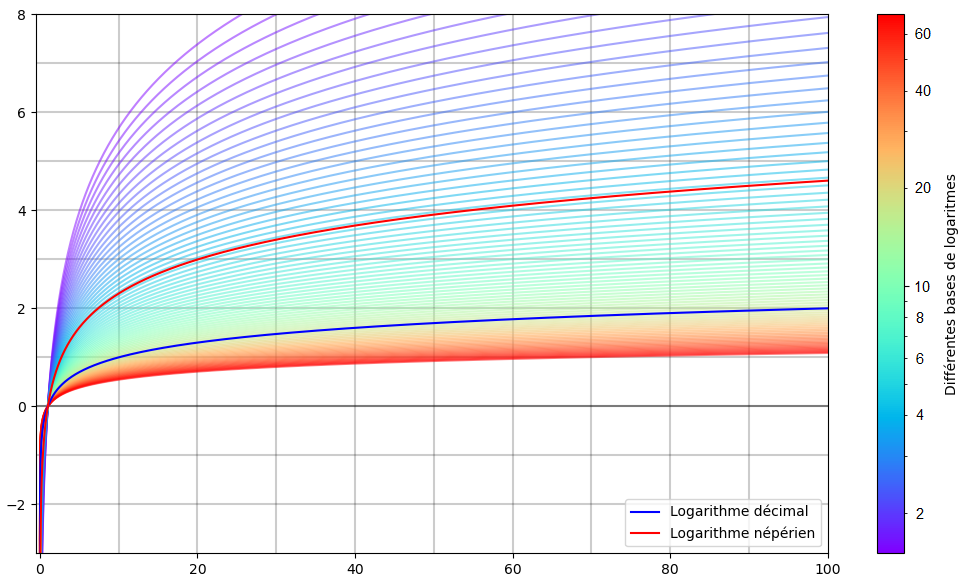
\includegraphics[scale=0.6]{log.png}}\\
	\vspace{0.15cm}
	{\noindent 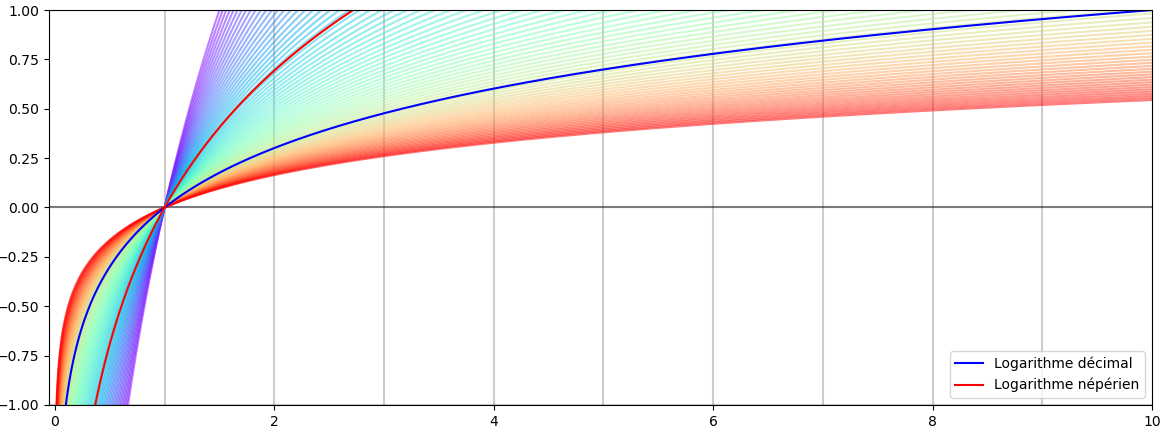
\includegraphics[scale=0.5]{log_zoom.png}}

	\newpage

	\subsection{Lecture de la table}

	La table donne, pour les réels compris entre $\numprint{1.0000}$ et $\numprint{9.9999}$, les $9$ premières décimales de leur logarithmes décimaux. Sa précision est très élevée, en pratique 4 à 5 décimales peuvent suffire.

	$\forall x \in [1, 10[,~\log(x) \in [0, 1[$, c'est pour cela que seules les décimales sont affichées.\\

	{ \parindent = 0 cm

	Concrètement, comment faire pour trouver le logarithme de, par exemple $\numprint{27.148}$ ?

	\vspace{0.2 cm}

	\begin{tabular}{lc|c}

	On factorise ce nombre : & $\numprint{27.148} = 10 \times \numprint{2.7148}$ & \\


	Première propriété : & $\log(\numprint{27.148}) = \log(10) + \log(\numprint{2.7148})$ & $ \log_a ( x \times y ) = \log_a (x) + \log_a (y) $\\

	& $\log(\numprint{27.148}) =1 + \log(\numprint{2.7148})$ & $ \log (10) = 1 $\\

	&& \\

	\multicolumn{2}{l|}{ \textit{Mais combien vaut le logarithme de $\mathit{\numprint{2.7148}}$ ?} } &\\


	\multicolumn{2}{l|}{ Pour le savoir, on découpe le nombre comme ceci : $2,714~|~8$} & \\



	\multicolumn{2}{l|}{On recherche la ligne $\mathbf{\numprint{2,741}}$ et on lit la valeur de la colonne $\mathbf{8}$} & (c'est à dire la $9^{\text{ème}}$ colonne)\\


	On sait maintenant que : & $\log (\numprint{2.7148}) = \numprint{0.433 737 841}$ & \\

	\multicolumn{3}{c}{} \\

	\multicolumn{3}{c}{\large $\log(\numprint{27.148}) = 1 + \numprint{0.433 737 841} = \mathbf{\numprint{1.433 737 841}} $}\\

	\end{tabular}
	}

	\vspace{0.3 cm}

	{ \parindent = 0 cm

	Un logarithme est composé de 2 parties :

	\begin{itemize}

		\vspace{0.1 cm}

		\item[•] La partie entière ($1$), qui indique l'ordre de grandeur du nombre (ici il est compris entre 10 et 100). On appelle ce nombre la \textbf{\textit{caractéristique}}.

		\vspace{0.1 cm}

		\item[•] La partie décimale ($\numprint{433 737 841}$), qui porte le nom de \textbf{\textit{mantisse}} et qui est lue dans la table.

	\end{itemize}
	}

	\vspace{0.3 cm}

	Cette table peut aussi être utilisée dans l'autre sens, si l'on cherche la valeur $x$ tel que $\log(x) = \numprint{0.763 240 757}$ ou, autrement dit la valeur de $10^{\numprint{0.763 240 757}}$, il faut trouver le nombre tel que son logarithme décimal vaille à $\numprint{0.763 240 757}$. Il suffit donc de parcourir la table (où les valeurs croissent au fur et à mesure de la descente) et de chercher ! \textit{Dans cet exemple, $\mathit{x}$ vaut $\mathit{\numprint{5.7975}}$.}

	\vspace{0.2 cm}

	\subsection{Cologarithme}

	Le Cologarithme sert à simplifier toujours plus les calculs, son but est de transformer les soustraction de logarithmes en addition de logarithmes.

	\begin{center}
	\begin{tabular}{ccl}

		$ \log_a \Big( \frac{1}{x} \Big) = - \log_a (x) $ & $ = $ & $\operatorname{colog}_a (x) $ \\
		
	\end{tabular}
	\end{center}

	On définit le cologarithme de la manière suivante :
	\begin{itemize}
		\item[•] On change le signe de la caractéristique et on soustrait $1$ à cette nouvelle caractéristique.
		\item[•] Si la caractéristique est négative, on change sa notation pour passer de $-x$ à $\overline{x}$. 
		\item[•] On retranche tous les chiffres de la mantisse à 9 et le dernier de droite à 10.
	\end{itemize}

	\vspace{2 mm}

	Dans cette écriture, la \textit{mantisse} est positive et la \textit{caractéristique} est algébrique. Son signe est indiqué (lorsqu'il est négatif) au-dessus. Lorsqu'on effectue un calcul, on fait toujours la somme (arithmétique) des mantisses et la somme algébrique des caractéristiques.\footnote{Démonstrations des propriétés des cologarithmes disponibles en \textbf{Annexe} (page \pageref{demo_colog})}

	\vspace{2 mm}

	{ \parindent=0cm Exemple : }

	\begin{tabular}{cl|cl}
		$\log \Big( \frac{1}{72} \Big) $ & $= \operatorname{colog} (72)$ & $~~\log \Big(38 \times \frac{1}{72} \Big)$ & $= \log(38) - \log(72)$\\
		
	$ \log (72) $ & $= 1,\numprint{857 332 496}$ & & $= \log(38) + \operatorname{colog}(72)$ \\

	$ \operatorname{colog} (72) $ & $= \overline{2},\numprint{142 667 504} $ & & $= \numprint{1.579 783 596} + \overline{2},\numprint{142 667 504}$\\

	& & & $= \numprint{1.579 783 596} -2 + \numprint{0.142 667 504}$\\

	& & & $= (1-2) + \numprint{0.579 783 596} + \numprint{0.142 667 504}$\\

	&&& $= \numprint{-1.722451100}$\\

	$10^{\numprint{-1.722451100}}$ & $= 0,1 \times \numprint{5,2778}$ & $38 \times \frac{1}{72}$ & $= \numprint{0,52778}$\phantom{$\numprint{7777}$} \textit{(Valeur calculée)}\\

	&&& $= \numprint{0.527 777 778}$ \textit{(Véritable valeur)}\\

	\end{tabular}





	\newpage

	\subsection{Utilisation des logarithmes pour réaliser des calculs}

	Les logarithmes nous permette de simplifier les calculs de produit et de quotient grâce aux propriétés vu dans la partie précédente. Pour cela, on va suivre une démarche que l'on retrouve beaucoup en Mathématique : Le théorème du parapluie.

	Pour marcher sous la pluie en restant sec, on peut utiliser un parapluie. Mais attention, pour rester bien sec, il faut l'utiliser astucieusement !

	\vspace{-0.15cm}

	\begin{center}
		\noindent {\small Départ en intérieur} $\xrightarrow{\text{Ouverture du parapluie}}$ {\small Marche sous la pluie} $\xrightarrow{\text{Fermeture du parapluie}}$ {\small Arrivée en intérieur}\\
	\end{center}

	\vspace{0.1cm}

	On va ici faire de même pour réaliser notre calcul : 

	\vspace{-0.15cm}

	\begin{center}
		\noindent {\small Calcul initial complexe} ~ $\xrightarrow{\log(x)}$ ~ {\small Calcul simplifié} ~ $\xrightarrow{10^x}$ ~ {\small Résultat du calcul initial}\\
	\end{center}

	\vspace{1cm}

	{\parindent = 0cm

	\underline{\textit{Calcul d'un produit} :} $\numprint{254860} \times \numprint{89642}$
	\vspace{0.2cm}

	\begin{large}
	\begin{tabular}{l|l}

	$= 10 ^{ \log ( \numprint{254860} ) } \times 10 ^ { \log ( \numprint{89642} ) }$ & \small Transformation du produit \\
	$= 10 ^{ \log ( \numprint{254860} ) + \log ( \numprint{89642} ) }$ & \small Regroupement des puissances\\
	$= 10 ^{ \log ( \numprint{100000} \times \numprint{2.54860}) + \log (\numprint{10000} \times \numprint{8.9642})}$ & \small Séparation des facteurs\\
	$= 10 ^{ \log(\numprint{100000}) + \log ( \numprint{2.54860} ) + \log(\numprint{10000}) + \log (\numprint{8.9642}) }$ & \small $ \log_a ( x \times y ) = \log_a (x) + \log_a (y) $\\
	$= 10 ^{ 5 + \log ( \numprint{2.54860} ) + 4 + \log ( \numprint{8.9642} ) }$ & \\
	$\approx 10 ^{ 5 + \numprint{0.406301679} + 4 + \numprint{0.952511538} }$ & \small \underline{\textbf{Lecture de la table}}\\
	$= 10 ^{ \numprint{10.358813217} }$ & \\
	$= 10 ^{ 10 } \times 10^{ \numprint{0.358813217} }$ & \small Séparation des puissances \\
	$\approx \numprint{10000000000} \times \numprint{2.2846}$ & \small \underline{\textbf{Lecture inversée de la table}} \\
	\\
	$\numprint{254860} \times \numprint{89642} \approx \numprint{22846000000} $ & \small Valeur calculée\\
	$\numprint{254860} \times \numprint{89642} = \numprint{22846160120} $ & \small Véritable valeur \\

	\end{tabular}
	\end{large}

	\vfill

	\underline{\textit{Calcul d'un quotient} :} $\numprint{55464} \div \numprint{34541}$
	\vspace{0.2cm}

	\begin{large}
	\begin{tabular}{l|l}

	$= 10 ^{ \log ( \numprint{55464} ) } \div 10 ^ { \log ( \numprint{34541} ) }$ & \small Transformation du quotient \\
	$= 10 ^{ \log ( \numprint{55464} ) - \log ( \numprint{34541} ) }$ & \small Regroupement des puissances\\
	$= 10 ^{ \log ( \numprint{10000} \times \numprint{5.5464}) - \log (\numprint{10000} \times \numprint{3.4541})}$ & \small Séparation des facteurs\\
	$= 10 ^{ \log(\numprint{10000}) + \log ( \numprint{5.5464} ) - (\log(\numprint{10000}) + \log (\numprint{3.4541})) }$ & \small $ \log_a ( x \times y ) = \log_a (x) + \log_a (y) $\\
	$= 10 ^{ 4 + \log ( \numprint{5.5464} ) - 4 - \log ( \numprint{3.4541} ) }$ & \\
	$= 10 ^{ 4 + \log ( \numprint{5.5464} ) - 4 + \operatorname{colog}( \numprint{3.4541} ) }$ & \small $\mathit{log( \numprint{3.4541} ) = \numprint{0.538334907}}$\\
	$\approx  10 ^{ (4 - 4) + \numprint{0.744011187}  + \overline{1},\numprint{461 665 093}}$ & \small \underline{\textbf{Lecture de la table}}\\
	$= 10 ^{ (4 - 4 - 1) + \numprint{0.744 011 187} +\numprint{0.461 665 093}}$ & \\
	$= 10 ^{ (-1) + \numprint{1.205 676 280} }$ & \\
	$= 10 ^{ 0 } \times 10^{ \numprint{0.205 676 280} }$ & \small Séparation des puissances \\
	$\approx  \numprint{1} \times \numprint{1.6057}$ & \small \underline{\textbf{Lecture inversée de la table}} \\
	\\
	$\numprint{55464} \div \numprint{34541} \approx  \numprint{1.605 7} $       & \small Valeur calculée  \\
	$\numprint{55464} \div \numprint{34541} = \numprint{1.605 743 899} $ & \small Véritable valeur \\

	\end{tabular}
	\end{large}

	\vfill

	}

	\newpage

	{\parindent = 0cm

	\underline{\textit{Calcul d'une puissance} :} $\numprint{68.453}^{\numprint{17}}$
	\vspace{0.2cm}

	\begin{large}
	\begin{tabular}{l|l}

	$= 10 ^{\log ( \numprint{68.453}^{\numprint{17}} ) }$ & \small Transformation de la puissance \\
	$= 10 ^{17 \times \log ( \numprint{68.453} ) }$ & \small $ \log_a ( x^n ) = n \log_a (x) $ \\
	$= 10 ^{17 \times \log ( \numprint{10} \times \numprint{6.8453} ) }$ & \small Séparation des facteurs\\
	$= 10 ^{17 \times (\log ( \numprint{10}) + \log (\numprint{6.8453} ))} $ & \small $ \log_a ( x \times y ) = \log_a (x) + \log_a (y) $\\
	$= 10 ^{17 \times 1 + 17 \times \log (\numprint{6.8453} )}$ & \\
	$\approx 10 ^{17 + 17 \times \numprint{0.835 392 486}}$ & \small \underline{\textbf{Lecture de la table}}\\
	$= 10 ^{17} \times 10^{10^{\log(17) + \log(\numprint{0.835 392 486})}}$ & \small Calcul du produit à l'aide de logarithmes\\
	$= 10 ^{17} \times 10^{10^{\log(10) + \log(1.7) + \log(0.1) + \log(\numprint{8.35392486})}}$ & \\
	$= 10 ^{17} \times 10^{10^{1 + \log(1.7) + (-1) + \log(\numprint{8.35 392 486})}}$ & \small $\log(\numprint{8.35 39}) = \numprint{0.921 889 272}$ \\
	$\approx 10 ^{17} \times 10^{10^{\numprint{0.230 448 921} + \numprint{0.921 889 272}}}$ & \small \underline{\textbf{2\up{ème} Lecture de la table}}\\
	$= 10 ^{17} \times 10^{10^{\numprint{1.152338193}}}$ & \\
	$= 10 ^{17} \times 10^{10^{1 + \numprint{.152338193}}}$ & \\
	$= 10 ^{17} \times 10^{10^1 \times 10^{\numprint{0.152 338 193}}}$ & \small $10^{\numprint{.152 349 508}} = \numprint{1.4202}$\\
	$\approx 10 ^{17} \times 10^{10 \times \numprint{1.4202}}$ & \small \underline{\textbf{Lecture inversée de la table}}\\
	$= 10 ^{17} \times 10^{\numprint{14.202}}$ & \\
	$= 10 ^{17} \times 10^{14 + \numprint{0.202}}$ & \\
	$= 10 ^{17} \times 10^{14} \times 10^{\numprint{0.202}}$ & \small $10^{\numprint{.202 024 895}} = \numprint{1.5923}$\\
	$\approx 10 ^{31} \times \numprint{1.5923}$ & \small \underline{\textbf{2\up{ème} Lecture inversée de la table}}\\
	\\
	$\numprint{68.453}^{\numprint{17}} \approx \numprint{1.592300000} \times 10^{31} $ & \small Valeur calculée\\
	$\numprint{68.453}^{\numprint{17}} = \numprint{1.591007637} \times 10^{31} $ & \small Véritable valeur \\

	\end{tabular}
	\end{large}
	}

	\vspace{0.3 cm}

	{\noindent\underline{\textit{Remarque} :}}

	\begin{itemize}

		\item[•] Ce calcul peut aussi s'appliquer au calcul de racine, car ~{\Large $\sqrt[]{x} = x^{\frac{1}{2}}$} et {\Large $\sqrt[3]{x} = x^{\frac{1}{3}}$}.
		
	\end{itemize}

	\vfill

	\subsubsection*{Analyse et Critique}

	Ces méthodes sont mathématiquement parfaitement véridiques, mais en pratique la table limite la précision des résultats obtenues. Si l'on reprend le calcul du produit $\mathit{\numprint{254860} \times \numprint{89642}}$, on remarque que le résultat n'est précis qu'à 5 chiffres près.

	La table, en lecture inversée, associe à chaque nombre entre $0$ et $1$ un autre nombre compris entre $1$ et $10$. Ce deuxième nombre n'est donné dans la table qu'avec 5 chiffres, c'est d'ici que provient le manque de précision du produit.

	En réalité : $10 ^{ 10 } \times 10^{\numprint{0.358813217}} = \numprint{22846160158.234503}$

	La précision est meilleure mais elle n'est pas parfaite non plus à cause de la première lecture du tableau, qui est limitée à 9 chiffres significatifs.\\


	\par Contrairement aux calculs de produit et de quotient, la méthode naïve consistant à utiliser un maximum de formule pour simplifier un maximum les calculs ne donne pas un résultat très précis pour calculer une puissance. Ici nous n'avons que 3 chiffres de juste, alors que précédemment, nous en avions 5 de correct.

	Ce manque de précision s'explique par les \textbf{4} approximations effectuées lors de la lecture de la table, et plus précisément par les lectures \textit{inverses}, et surtout par la toute dernière.\\

	\vfill

	\newpage







	\subsubsection*{Améliorer la précision des mesures}

	{\parindent = 0cm}

	Il existe quatre solutions pour obtenir des résultats plus précis :

	\begin{itemize}
		
		%\setlength{\itemindent}{-0.8 cm}	
		
		\vspace{0.2cm}
		
		\item[•] \textbf{Découper le calcul :}
		
		\begin{small}
		On peut séparer les facteurs de notre calcul en plus petits facteurs, reprenons l'exemple du calcul du produit $\mathit{\numprint{254860} \times \numprint{89642}}$:\\
		
		\vspace{-2mm}
		\begin{itemize}
		
			%\setlength{\itemindent}{-0.4 cm}	
			
			\item[] $= (254 \cdot 10^{3} + 860) \times (89 \cdot 10^{3} + 642)$
			\vspace{0.1 cm}
			\item[] $= (254 \cdot 10^{3})(89 \cdot 10^{3}) + (254 \cdot 10^{3})(642) + (860)(89 \cdot 10^{3}) + (860)(642)$
			\vspace{0.1 cm}
			\item[] $= (254)(89)\cdot 10^{6} + \big[(254)(642) + (860)(89)\big] \cdot 10^{3} + (860)(642)$
			\vspace{0.1 cm}
			\item[] $= 10^{\log(254)+\log(89)} \cdot 10^{6} + \big[10^{\log(254)+\log(642)} + 10^{\log(860)+\log(89)}\big] \cdot 10^{3} + 10^{\log(860)+\log(642)}$
			\vspace{0.1 cm}
			\item[] $= 10^{\numprint{2.404833717}+\numprint{1.949390007}} \cdot 10^{6}$\\
			$\phantom{=} + \big[10^{\numprint{2.404833717}+\numprint{2.807535028}} + 10^{\numprint{2.934498451}+\numprint{1.949390007}}\big] \cdot 10^{3}$\\
			$\phantom{=} + 10^{\numprint{2.934498451}+\numprint{2.807535028}}$
			\vspace{0.1 cm}
			\item[] $= 10^{\numprint{4.354223724}} \cdot 10^{6} + \big[10^{\numprint{5.212368745}} + 10^{\numprint{4.883888458}}\big] \cdot 10^{3} + 10^{\numprint{5.742033479}}$
			\vspace{0.1 cm}
			\item[] $= 10^{\numprint{0.354223724}} \cdot 10^{10} + \big[10^{\numprint{1.212368745}} + 10^{\numprint{0.883888458}}\big] \cdot 10^{7} + 10^{\numprint{0.742033479}} \cdot 10^{5}$
			\vspace{0.1 cm}
			\item[] $= \numprint{2.2606} \cdot 10^{10} + \big[\numprint{16.307} + \numprint{7.6540}\big] \cdot 10^{7} + \numprint{5.5212} \cdot 10^{5}$
			\vspace{0.1 cm}
			\item[] $= \numprint{2.2606} \cdot 10^{10} + \numprint{23.961} \cdot 10^{7} + \numprint{5.5212} \cdot 10^{5}$
			\vspace{0.2 cm}
			\item[] $= \numprint{22846162120}$ (Valeur calculée)
			\vspace{0.1 cm}
			\item[] $= \numprint{22846160120}$ (Véritable valeur)\\
		\end{itemize}
		
		Pour améliorer la précision, il est possible de découper encore plus les facteurs du calcul.
		
		\end{small}

		
		\vfill
		
		\item[•] \textbf{Lire entre les lignes :} 
		
		{\small On peut approximer la valeur d'un logarithme en supposant localement qu'il évolue linéairement. Pour avoir plus de détail, rendez-vous dans la section correspondante (page \pageref{approximation_lineaire}).}
		
		\vfill
		
		\item[•] \textbf{Pourquoi faire simple :} 
		
		\begin{small}
		Dans le cas du calcul de la puissance, on aurait aussi pu se contenter de faire la multiplication $\mathit{17 \times \numprint{0.835392486} }$ manuellement, on peut se satisfaire d'avoir transformer notre puissance complexe en multiplication plus simple :
		\vspace{0.1cm}
		
		\begin{itemize}
			\item[] $= 10^{17 + 17 \times \numprint{0.835 392 486}}$
			\item[] $= 10^{17 + \numprint{14.201672262}}$
			\item[] $= 10^{31} \times 10^{\numprint{0.201672262}}$
			\item[] $= \numprint{1.5910} \times 10 ^{31}$
		\end{itemize}
		\end{small}
		
		\vfill
		
		\item[•] \textbf{Faire autrement :} 
		
		{\small Il existe d'autres méthodes pour calculer des puissances, comme par exemple l'Exponentiation rapide (cette méthode est détaillée à la page \pageref{exponentiation_rapide})}

	\end{itemize}

	\vfill

	{\noindent\underline{\textit{Remarque} :}}\\

	\vspace{-2mm}
	Les calculs présentés sont des exemples simples bien choisis, avec des nombres n'ayant que 5 chiffres, ce qui correspond (comme par hasard) à la précision de la table.
		\begin{center}
		Donc comment faire si les nombres que l'on manipule ont plus de 5 chiffres ?
		\end{center}
		
		On peut décomposer les facteurs en plus petits facteurs : 
		
		\vspace{2 mm}	
		
		$ \numprint{1 554 548 431} \times \numprint{6 224 814 231}$
		
		\vspace{0.1cm}
		\begin{small}
		\begin{itemize}
			\item[] $= (\numprint{15545} \cdot 10^5 + \numprint{48 431}) \times (\numprint{62248} \cdot 10^5 + \numprint{14 231}) $
			\vspace{0.1 cm}
			\item[] $= (\numprint{15545} \cdot 10^5) (\numprint{62248} \cdot 10^5) + (\numprint{15545} \cdot 10^5) (\numprint{14 231}) + (\numprint{48 431}) (\numprint{62248} \cdot 10^5) + (\numprint{48 431}) (\numprint{14 231})$
			\vspace{0.1 cm}
			\item[] $= (\numprint{15545}) (\numprint{62248}) \cdot 10^{10} + \big[(\numprint{15545})(\numprint{14 231}) + (\numprint{48 431}) (\numprint{62248})\big] \cdot 10^5 + (\numprint{48 431}) (\numprint{14 231})$
			\vspace{0.1 cm}
			\item[] $= \numprint{967640000} \cdot 10^{10} + \big[\numprint{221220000} + \numprint{3014700000}\big] \cdot 10^5 + \numprint{689220000}$
			\vspace{3 mm}
			\item[] $= \numprint{9676723592689220000}$ (Valeur calculée)
			\vspace{0.1 cm}
			\item[] $= \numprint{9676775196067521561}$ (Véritable valeur)
		\end{itemize}
		\end{small}

	\vfill

	\newpage

	\subsection{Approximation linéaire du logarithme}\label{approximation_lineaire}

		À l'aide de la table et de quelques calculs, on peut approximer des logarithmes de nombre ayant plus de 5 décimales. Pour cela, on suppose que l'évolution entre deux logarithmes déjà connus est linéaire.
		
		Sur les courbes ci-dessous, les points rouges représentent les valeurs calculées dans la table, et la courbe bleue est la courbe exacte du logarithme décimale.

	\vspace{-1 mm}

	\begin{center}
		{              \noindent 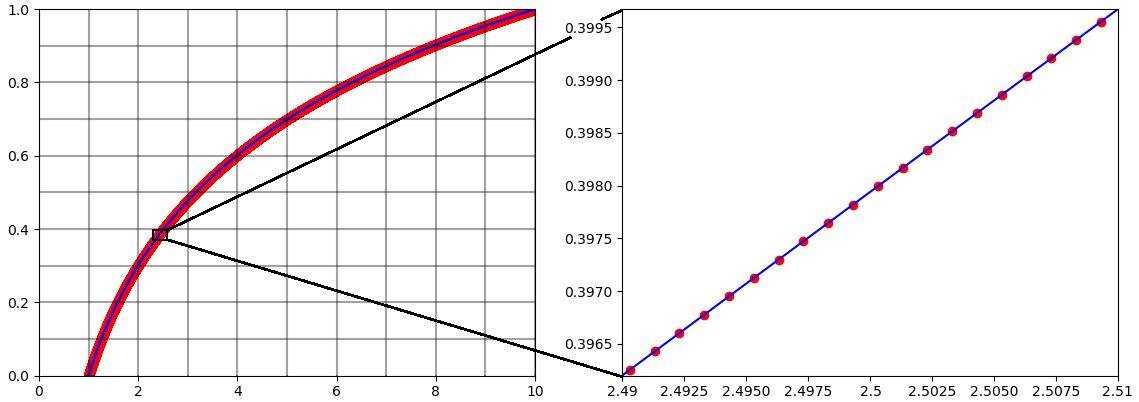
\includegraphics[scale = 0.45]{Approx log zoom.png } }
		
		{\vspace{3 mm} \noindent 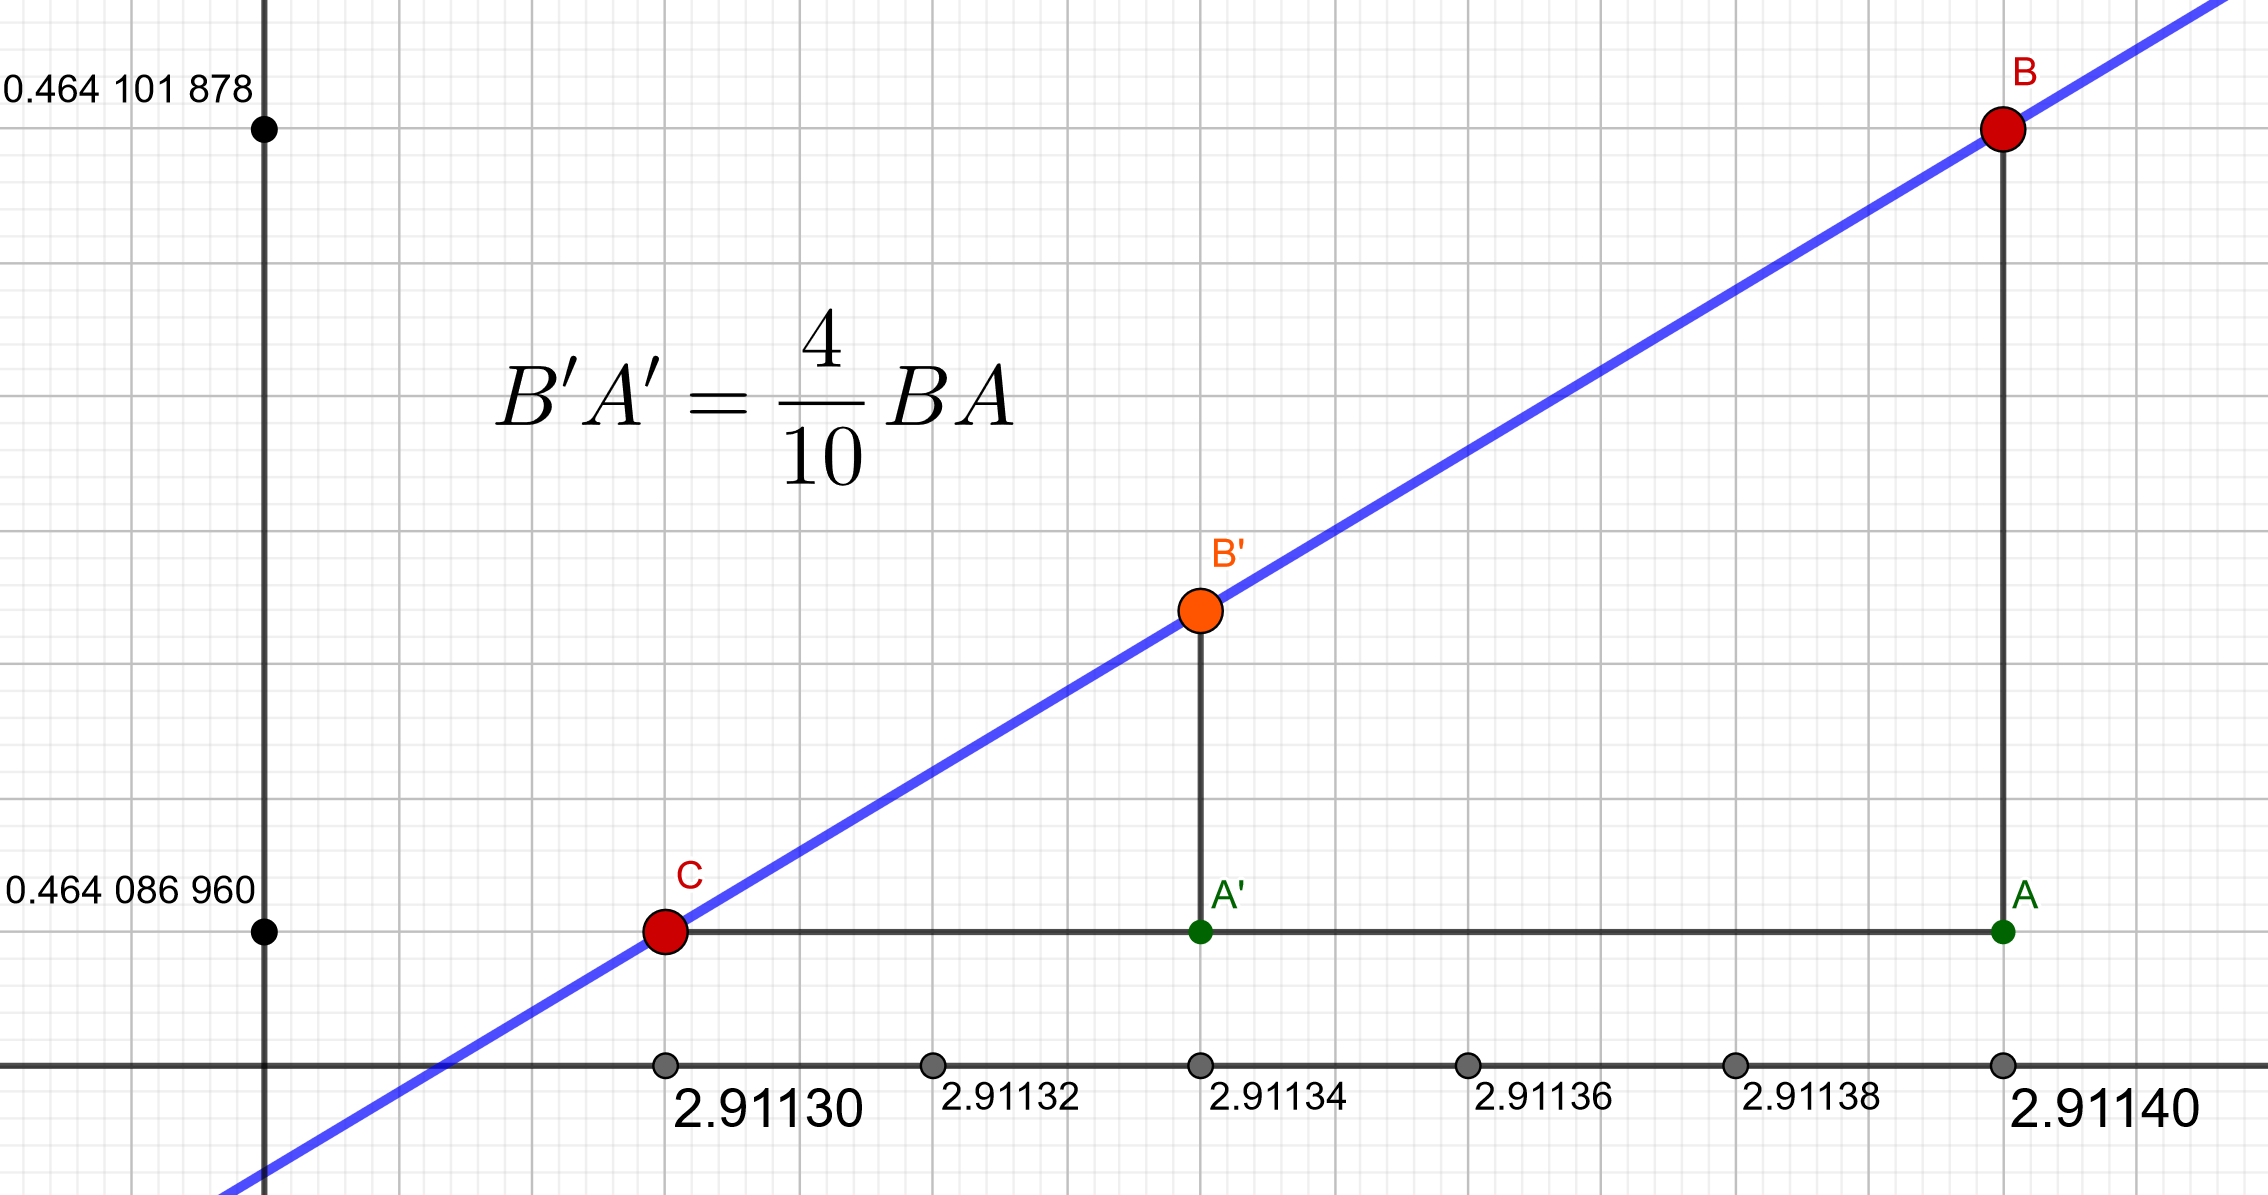
\includegraphics[scale = 0.225]{Log/Log Geogebra.png} }
	\end{center}

	Pour calculer cette approximation, on peut utiliser le théorème de Thalès.

	\vspace{1 mm}

	{\noindent Calculons par exemple : $\log(\numprint{2.91134})$}

	\vspace{1 mm}

	{\parindent = 0cm

	\begin{small}
	\begin{tabular}{cl|l}
	$\log (\numprint{2.91134}) $ & $\approx \log ( \numprint{2.91130} ) + \frac{4}{10} \times ( \log ( \numprint{2.91140} ) - \log ( \numprint{2.91130} ) )$ & Théorème de Thalès\\
								& $\approx \numprint{0.464 086 960} + 10^{-1} \times 4 \times (\numprint{0.000014 918} )$ & \underline{\textbf{Lecture de la table}}\\
								& $= \numprint{0.464 086 960} + 10^{-6} \times 4 \times ( \numprint{1.4 918} )$ &\\
								& $= \numprint{0.464 086 960} + 10^{-6} \times 10^{\log(4)~+~\log(\numprint{1.4 918})}$ & Calcul du produit\\
								& $\approx \numprint{0.464 086 960} + 10^{-6} \times 10^{\numprint{0.602 059 991}~+~\numprint{0.173 710 603}}$ &\\
								& $= \numprint{0.464 086 960} + 10^{-6} \times 10^{\numprint{0.775770594}}$ & \\
								& $\approx \numprint{0.464 086 960} + \numprint{0.000 005 967 2}$ & \underline{\textbf{Lecture de la table}}\\
								& & \\
								& $= \numprint{0.464 092 927 2} \rightarrow $ $10^{\numprint{0.464 092 927 2}} = \numprint{2.911 339 998 953}$ & Valeur calculée \\
								& $= \numprint{0.464 092 927 4} \rightarrow $ $10^{\numprint{0.464 092 927 4}} = \numprint{2.911 340 000 294}$  & Véritable valeur\\
	\end{tabular}
	\end{small}

	}

	\vspace{2 mm}

	Il est possible d'utiliser cette approximation dans l'autre sens, c'est à dire de trouver la valeur de, par exemple $10^{\numprint{0.845 672 172}}$. Dans la table, on peut lire : $\numprint{7.0092} <  10^{\numprint{0.845 672 172}} < \numprint{7.0093}$.

	\vspace{2 mm}

	{\parindent = 0cm

	On cherche donc un réel $x$, tel que $10^{\numprint{0.845 672 172}} = \numprint{7.0092} + 10^{-5} \times x$

	\vspace{3 mm}

	\begin{small}
	\begin{tabular}{cl|l}
	$\log (10^{\numprint{0.845 672 172}}) $ & $\approx \log ( \numprint{7.00920} ) ~ + $ {\large$\frac{x}{10}$} $ \times ~ ( \log ( \numprint{7.00930} ) - \log ( \numprint{7.00920} ) )$ & Théorème de Thalès\\

	&& \\

	$\numprint{0.845 672 172}$	 & $\approx \numprint{0.845 668 452} + 10^{-1} \times x \times (\numprint{0.845 674 648} - \numprint{0.845 668 452} )$ & \underline{\textbf{Lecture de la table}}\\

								& $\approx \numprint{0.845 668 452} + x \times \numprint{0.000 000 619 6}$ & \\
								
	&& \\

	$x$&$=$ {\normalsize$\frac{\numprint{0.845 672 172} -  \numprint{0.845 668 452}} {\numprint{0.000 000 619 6}} $} $=$ {\normalsize$\frac{\numprint{0.000 003 720 0}} {\numprint{0.000 000 619 6}} $} $=$ {\normalsize$\frac{\numprint{3 7200}} {\numprint{619 6}} $} $= \cdots$  & Calcul du quotient \\
								
								& $\approx \numprint{6.0039}$ & \underline{\textbf{Lecture de la table}}\\
								
	&& \\
								
	$10^{\numprint{0.845 672 172}}$ & $= \numprint{7.0092} + 10^{-5} \times \numprint{6.0039}$ & \\
									& $= \numprint{7.009 260 039}$ & Valeur calculée\\
									& $= \numprint{7.009 260 034}$ & Véritable valeur\\
	\end{tabular}
	\end{small}

	}

	\newpage

	\subsection{Changement de base de Logarithme}

	Comme vu dans la présentation du logarithme népérien, il est possible de passer d'une base à une autre grâce à cette formule : 
	\begin{center}
	\begin{LARGE}

		$ \log_a (x) = \frac{\ln (x)}{\ln (a)}$ 
		
	\end{LARGE}
	\end{center}

	\begin{center}
	Mais comme vous le savez, les logarithmes de la table sont dans la base décimale !

	Donc comment faire pour obtenir un logarithme dans une autre base ?
	\end{center}

	Facile, il suffit d'adapter la formule vue plus haut :

	\vspace{0.1cm}

	\begin{large}
	\begin{center}
		$ \log_a (x) = \frac{\ln (x)}{\ln (a)} ~~~ \Longleftrightarrow ~~~ \ln (x) = \log_a (x) \times \ln (a)$\\ 

	\end{center}
	\end{large}

	Ce résultat est vrai pour toutes les bases, y compris la base décimale, on sait donc que :

	\vspace{0.1cm}

	\begin{large}
	\begin{center}

		$ \ln (x) = \log_{10} (x) \times \ln (10)$\\ 
		
	\end{center}
	\end{large}

	On peut donc remplacer $\ln (x)$ :

	\begin{LARGE}
	\begin{center}

		{\large $ \log_a (x) \times \ln (a) = \log_{10} (x) \times \ln (10) ~~ \Longleftrightarrow ~~ \log_a (x) = \log_{10} (x) \times \frac{\ln(10)}{\ln(a)} ~~ \Longleftrightarrow $ }\\
		\vspace{0.2cm}
		$\log_a (x) ~ = ~ \frac{\log_{10} (x)}{\log_{10} (a)} ~ = ~ 10^{\log(\log_{10} (x))~-~\log(\log_{10} (a))}$\\ 
		
	\end{center}
	\end{LARGE} 

	\vspace{0.2cm}

	\begin{center}
	\begin{large}
	\begin{tabular}{c||l||l|l}

	\Large $a$ & \LARGE \hfil $ \frac{1}{\log_{10}(a)} $ \hfill & \Large \hfil $\log(\ln(a))$ \hfill & \Large \hfil  $- \log(\log_{10}(a))$ \hfill \\

	&&&\\

	$2$ & $\numprint{3.321928094887362}$ & $ \numprint{-0.159174538954862}$ & $ \phantom{-}\numprint{0.521390227654325} $\\

	$2.5$ & $\numprint{2.512941594732060}$ & $ \numprint{-0.037966706228034}$ & $ \phantom{-}\numprint{0.400182394927497} $\\

	$\mathbf{e}$ & $\numprint{2.302585092994046}$ & $ \phantom{-}\numprint{0}$ & $ \phantom{-}\numprint{0.362215688699463} $\\

	$3$ & $\numprint{2.095903274289385}$ & $ \phantom{-}\numprint{0.040844452568921}$ & $ \phantom{-}\numprint{0.321371236130543} $\\

	$4$ & $\numprint{1.660964047443681}$ & $ \phantom{-}\numprint{0.141855456709120}$ & $ \phantom{-}\numprint{0.220360231990344} $\\

	$5$ & $\numprint{1.430676558073393}$ & $ \phantom{-}\numprint{0.206674227491119}$ & $ \phantom{-}\numprint{0.155541461208344} $\\

	$6$ & $\numprint{1.285097208938469}$ & $ \phantom{-}\numprint{0.253279708340476}$ & $ \phantom{-}\numprint{0.108935980358987} $\\

	$7$ & $\numprint{1.183294662454938}$ & $ \phantom{-}\numprint{0.289122783172642}$ & $ \phantom{-}\numprint{0.073092905526821} $\\

	$8$ & $\numprint{1.107309364962454}$ & $ \phantom{-}\numprint{0.317946715764801}$ & $ \phantom{-}\numprint{0.044268972934662} $\\

	$9$ & $\numprint{1.047951637144692}$ & $ \phantom{-}\numprint{0.341874448232902}$ & $ \phantom{-}\numprint{0.020341240466561} $\\

	$10$ & $\numprint{1}$ & $ \phantom{-}\numprint{0.362215688699463}$ & $ \phantom{-}\numprint{0} $\\

	$11$ & $\numprint{0.960252567789128}$ & $ \phantom{-}\numprint{0.379830211523892}$ & $ \numprint{-0.017614522824429} $\\

	$12$ & $\numprint{0.926628408029127}$ & $ \phantom{-}\numprint{0.395310078283252}$ & $ \numprint{-0.033094389583789} $\\

	$13$ & $\numprint{0.897711717502623}$ & $ \phantom{-}\numprint{0.409078794792035}$ & $ \numprint{-0.046863106092572} $\\

	$14$ & $\numprint{0.872502869549156}$ & $ \phantom{-}\numprint{0.421448824727484}$ & $ \numprint{-0.059233136028021} $\\

	$15$ & $\numprint{0.850274153727603}$ & $ \phantom{-}\numprint{0.432656710921376}$ & $ \numprint{-0.070441022221913} $\\

	$16$ & $\numprint{0.830482023721841}$ & $ \phantom{-}\numprint{0.442885452373101}$ & $ \numprint{-0.080669763673638} $\\

	$17$ & $\numprint{0.812711509291959}$ & $ \phantom{-}\numprint{0.452279278600139}$ & $ \numprint{-0.090063589900676} $\\

	$18$ & $\numprint{0.796639770196912}$ & $ \phantom{-}\numprint{0.460953705047035}$ & $ \numprint{-0.098738016347571} $\\

	$19$ & $\numprint{0.782011483099541}$ & $ \phantom{-}\numprint{0.469002558388783}$ & $ \numprint{-0.106786869689320} $\\

	$20$ & $\numprint{0.768621786840241}$ & $ \phantom{-}\numprint{0.476502998175098}$ & $ \numprint{-0.114287309475634} $\\

	\end{tabular}
	\end{large}
	\end{center}


	\newpage

	\section{Exponentiation Rapide} \label{exponentiation_rapide}

	Pour calculer la puissance $n^p$, la méthode naïve et immédiate est de multiplier $n$ par lui-même $p$ fois. Cependant, il existe des méthodes plus efficaces, où le nombre d'opérations nécessaires n'est plus de l'ordre de $p$ mais de l'ordre de $\log(p)$.

	On peut réécrire l'exposant $p$ en somme de plus petits exposants de cette manière :

	{\noindent $ p=\sum\limits_{i\leq d}a_{i}2^{i} $ avec $ a_{i}\in \{0,1\} $, on constate que :}

	\vspace{-2mm}

		$$n^{p} = (n^{2^{0}})^{{a_{0}}} \times (n^{2^{1}})^{{a_{1}}} \times (n^{{2^{2}}})^{{a_{2}}} \times \dots \times (n^{{2^{d}}})^{{a_{d}}}.$$

	Il faut ainsi $d$ opérations pour calculer tous les $n^{2^{i}}$, puis $d$ opérations supplémentaires pour former le produit des $(n^{{2^{i}}})^{{a_{i}}}$. Le nombre total d'opérations est donc $2d$, qui est bien de l'ordre du logarithme de $p$. Cette simple remarque algébrique conduit à l'algorithme présenté dans la section suivante.

	\vfill

	\subsection*{Algorithme}

	Soit $n$ un entier strictement supérieur à 1, supposons que l'on sache calculer, pour chaque réel $x$, toutes les puissances $x^k$ de $x$, pour tout $k$, tel que $1 \leq k < n$.

	\vspace{1mm}

	\begin{itemize}

		\item[•] Si $n$ est pair alors $x^n = (x^2)^{\frac{n}{2}}$. Il suffit alors de calculer $y^{\frac{n}{2}}$ pour $y = x^2$.
		\item[•] Si $n$ est impair et $n > 1$, alors $x^n = x(x^2)^{\frac{n-1}{2}}$. Il suffit de calculer $y^{\frac{n-1}{2}}$ pour $y = x^2$ et de multiplier le résultat par $x$.

	\end{itemize}

	\vspace{2mm}

	Cette remarque nous amène à l'algorithme récursif suivant qui calcule $x^n$ pour un entier strictement positif $n$ :

	\vspace{-2mm}

		$${\mbox{{\LARGE $x^n$}}} = \left\{{   
		\begin{matrix}
		\vspace{2mm}
		{\mbox{{\Large $x$}}} & {\mbox{si $n = 1$}}\\
		\vspace{2mm}
		{\mbox{{\Large $(x^2)^{\frac{n}{2}}$}}} & {\mbox{si $n$ est pair}}\\
		{\mbox{{\Large $x \times (x^2)^{\frac{n-1}{2}}$}}} & {\mbox{si $n$ est impair}}\\
		\end{matrix}}\right.$$

	\vspace{2mm}

	En comparant à la méthode ordinaire qui consiste à multiplier $x$ par lui-même $n - 1$ fois, cet algorithme nécessite de l'ordre de $\mathrm{O}(\log n)$ multiplications et ainsi accélère le calcul de $x^n$ de façon spectaculaire pour les grands entiers.

	\vfill

	\subsection*{Exemple}

	{\parindent = 0cm

	Calculons $65^{27}$ :
	\vspace{0.2cm}

	\begin{large}
	\begin{tabular}{l|l}

	$= 65 \times (65^2)^{\frac{27-1}{2}}$ & \small $27$ est impair \\
	$= 65 \times (\numprint{4225})^{13}$ \\
	$= 65 \times \numprint{4225} \times (\numprint{4225}^2)^{\frac{13-1}{2}}$ & \small $13$ est impair \\
	$= 65 \times \numprint{4225} \times (\numprint{17850625})^{6}$ \\
	$= 65 \times \numprint{4225} \times (\numprint{17850625}^2)^{\frac{6}{2}}$ & \small $\phantom{0}6$ est pair \\
	$= 65 \times \numprint{4225} \times (\numprint{318644812890625})^{3}$ \\
	$= \numprint{8885065410379260901802741051591932773590087890625}$ \\

	\end{tabular}
	\end{large}
	}

	\vspace{3 mm}

	Comme on peut le voir avec cet exemple, la méthode fonctionne bien, mais elle est complexe à utiliser en pratique, surtout si l'exposant est grand. 
	Cette méthode est bien plus pratique pour un ordinateur, qui est bien plus à l'aise avec les multiplications qu'avec les puissances.

	Néanmoins en combinant cette méthode avec les logarithmes, on peut toujours plus simplifier les calculs.

	\vfill
	\vfill
	\vfill

	\newpage





	\section{Annexe}
	\subsection{Démonstration des Critères de Divisibilité de 2 à 10} \label{demo_1_a_10}

	\large

	\subsubsection*{Critère de Divisibilité par 2}

	\begin{center}
		{\LARGE $^2|_n$} $ ~~ \Longleftrightarrow ~~ \exists p \in \mathbb{Z}, ~~ n = 2p $\\
		
		\vspace{2mm}
		
		{\normalsize $ p_0 \in \{0,1,2,3,4,5,6,7,8,9\} ~~ \Longleftrightarrow ~~ n_0 \in \{ 0,2,4,6,8 \}$}\\
		
		\vspace{2mm}	
		
		{\LARGE $^2|_n$} $~~ \Longleftrightarrow ~~ n_0 \in \{ 0,2,4,6,8 \}$
		
	\end{center}



	\subsubsection*{Critère de Divisibilité par 3}

	\begin{center}
		{\LARGE $^3|_n$} $ ~~ \Longleftrightarrow ~~ \exists p \in \mathbb{Z}, ~~ n = 3p $\\
		
		\vspace{2mm}
			
		{\normalsize $ n = \sum\limits_{i=0}^k n_i \cdot 10^i = 3p ~~~ \Longleftrightarrow ~~~ p = \sum\limits_{i=0}^k n_i \cdot \frac{10^i}{3} ~ = ~ \sum\limits_{i=0}^k n_i \cdot \left( \frac{1}{3} + \frac{10^i-1}{3} \right) ~ = ~ \frac{1}{3} \sum\limits_{i=0}^k n_i + \sum\limits_{i=0}^k n_i \cdot \frac{10^i-1}{3}$}\\
		
		\vspace{2mm}
			
		{\Large $^3|_n$} {\normalsize $ ~~ \Longleftrightarrow ~~ p \in \mathbb{Z} ~~ \Longleftrightarrow ~~ \frac{1}{3}\sum\limits_{i=0}^k n_i + \sum\limits_{i=0}^k n_i \cdot \frac{10^i-1}{3} \in \mathbb{Z} ~~ \Longleftrightarrow ~~ \frac{1}{3}\sum\limits_{i=0}^k n_i \in \mathbb{Z}$ }
		
		\vspace{3mm}	
		
		{\LARGE $^3|_n$} $~ \Longleftrightarrow ~$ {\LARGE $^3|_{n_k ~ + ~ \dots ~ + ~ n_0}$}
		
	\end{center}



	\subsubsection*{Critère de Divisibilité par 4}

	\begin{center}
	\begin{tabular}{r|r|r}

		\multicolumn{3}{l}{\hspace{4.2 cm} {\LARGE $^4|_n$} $ ~~ \Longleftrightarrow ~~ n \equiv 0 ~~ [4] $ }\\
		
		\multicolumn{3}{c}{\vspace{-2 mm}} \\
		
		{\normalsize $\overline{n_{_{k}}~\dots~n_{_1}~n_{_0}} \equiv 0 ~~ [4]$} & {\normalsize $\overline{n_{_{k}}~\dots~n_{_2}} \cdot 100 + \overline{n_{_1}~n_{_0}} \equiv 0 ~~ [4]$} & {\normalsize $10 \cdot n_{_1} + n_{_0} \equiv 0 ~~ [4]$}\\
		
		{\normalsize $(8+2) \cdot n_{_1} + n_{_0} \equiv 0 ~~ [4]$} & {\normalsize $ 8 \cdot n_{_1} +2 \cdot n_{_1} + n_{_0} \equiv 0 ~~ [4]$} & {\normalsize $2 \cdot n_{_1} + n_{_0} \equiv 0 ~~ [4]$}\\
		
		\multicolumn{3}{c}{\vspace{-2 mm}} \\
		
		\multicolumn{3}{l}{\hspace{4.2 cm} {\LARGE $^4|_n$} $ ~~ \Longleftrightarrow ~~ $ {\LARGE $^4|_{2n_{_1} ~ + ~ n_{_0}}$} }\\
		
	\end{tabular}
	\end{center}



	\subsubsection*{Critère de Divisibilité par 5}

	\begin{center}

	\textit{{Démonstration analogue au Critère de Divisibilité par 2}}

	\end{center}



	\subsubsection*{Critère de Divisibilité par 6}

	\begin{center}

	{\LARGE $^6|_n$} $ ~~ \Longleftrightarrow ~~ $ {\LARGE $^{2~\times~3}|_n$} $ ~~ \Longleftrightarrow ~~ $ {\LARGE $^{2}|_n$ {\large et} $^{3}|_n$} 

	\end{center}



	\subsubsection*{Critère de Divisibilité par 8}

	\begin{center}
	\begin{tabular}{r|r|r}

		\multicolumn{3}{l}{\hspace{4.2 cm} {\LARGE $^8|_n$} $ ~~ \Longleftrightarrow ~~ n \equiv 0 ~~ [8] $ }\\
		
		\multicolumn{3}{c}{\vspace{-2 mm}} \\
		
		{\normalsize $\overline{n_{_{k}}~\dots~n_{_1}~n_{_0}} \equiv 0 ~~ [8]$} & {\normalsize $\overline{n_{_{k}}~\dots~n_{_3}} \cdot 1000 + \overline{n_{_2}~n_{_1}~n_{_0}} \equiv 0 ~~ [8]$} & {\normalsize $ 100 \cdot n_{_2} + 10 \cdot n_{_1} + n_{_0} \equiv 0 ~~ [8]$}\\
		
		\multicolumn{2}{c|}{\normalsize $(96 + 4) \cdot n_{_2} + (8+2) \cdot n_{_1} + n_{_0} \equiv 0 ~~ [8]$} &  {\normalsize $4 \cdot n_{_2} + \phantom{1}2 \cdot n_{_1} + n_{_0} \equiv 0 ~~ [8]$}\\
		
		\multicolumn{3}{c}{\vspace{-2 mm}} \\
		
		\multicolumn{3}{l}{\hspace{4.2 cm} {\LARGE $^4|_n$} $ ~~ \Longleftrightarrow ~~ $ {\LARGE $^4|_{4n_{_2} ~ + ~ 2n_{_1} ~ + ~ n_{_0}}$} }\\
		
	\end{tabular}
	\end{center}



	\subsubsection*{Critère de Divisibilité par 9}

	\begin{center}

	\textit{Démonstration analogue au Critère de Divisibilité par 3}

	\end{center}


	\newpage

	\subsubsection*{Critères de divisibilité par 7}

	{\normalsize Il existe plusieurs méthodes pour savoir si un nombre est divisible par 7. Celles qui sont présentées sont adaptées à différentes tailles de nombres.}

	\paragraph*{Première méthode}

	\begin{center}
		\huge
		$ ^{7}|_n \Leftrightarrow$ $^{7}|_{\overline{n_{_{k}}~\dots~n_{_2}~n_{_1}}~+~5n_{_0}} $
	\end{center}

	{\normalsize Démonstration :}

	\vspace{-0.6cm}

	\begin{center}
	\begin{tabular}{r|r|r}
		
		{\normalsize \hspace{-3 mm} $\overline{n_{_{k}} \dots n_{_1}~n_{_0}} \equiv 0 ~~ [7]$} & {\normalsize $10 \cdot \overline{n_{_{k}} \dots n_{_1}} + n_{_0} \equiv 0 ~~ [7]$} & {\normalsize $10 \cdot \overline{n_{_{k}} \dots n_{_1}} + 50 n_{_0} - 49 n_{_0} \equiv 0 ~~ [7]$}\\
		
		{\normalsize \hspace{-3 mm} $10 \cdot \overline{n_{_{k}} \dots n_{_1}} + 50 n_{_0} \equiv 0 ~~ [7]$} & {\normalsize $10 \cdot (\overline{n_{_{k}} \dots n_{_1}} + 5 n_{_0}) \equiv 0 ~~ [7]$} & {\normalsize $\overline{n_{_{k}} \dots n_{_1}} + 5 n_{_0} \equiv 0 ~~ [7]$}\\
		
	\end{tabular}
	\end{center}

	\vspace{3 mm}



	\paragraph*{Deuxième méthode}

	\begin{center}
		\huge
		$ ^{7}|_n \Leftrightarrow$ $^{7}|_{\overline{n_{_{k}}~\dots~n_{_2}~n_{_1}}~-~2n_{_0}} $
	\end{center}

	{\normalsize Démonstration :}

	\vspace{-0.6cm}

	\begin{center}
	\begin{tabular}{r|r|r}
		
		{\normalsize \hspace{-3 mm} $\overline{n_{_{k}} \dots n_{_1}~n_{_0}} \equiv 0 ~~ [7]$} & {\normalsize $10 \cdot \overline{n_{_{k}} \dots n_{_1}} + n_{_0} \equiv 0 ~~ [7]$} & {\normalsize $10 \cdot \overline{n_{_{k}} \dots n_{_1}} - 20 n_{_0} + 21 n_{_0} \equiv 0 ~~ [7]$}\\
		
		{\normalsize \hspace{-3 mm} $10 \cdot \overline{n_{_{k}} \dots n_{_1}} - 20 n_{_0} \equiv 0 ~~ [7]$} & {\normalsize $10 \cdot (\overline{n_{_{k}} \dots n_{_1}} - 2 n_{_0}) \equiv 0 ~~ [7]$} & {\normalsize $\overline{n_{_{k}} \dots n_{_1}} - 2 n_{_0} \equiv 0 ~~ [7]$}\\
		
	\end{tabular}
	\end{center}

	\vspace{3 mm}



	\subsubsection*{Troisième méthode \textit{(Critère pour un grand nombre)}}

	\begin{normalsize}
		Pour les grands nombres, la méthode du Ruban de Pascal est la plus pratique pour savoir si un nombre est divisible par 7, pour avoir plus de détail, rendez-vous à la page \pageref{subsection_critere_10_plus_ou_moins_1}.
		
	\begin{center}
		\huge
		$ ^{7}|_n \Leftrightarrow$ $^{7}|_{\overline{n_{_{k}}~n_{_{k-1}}~n_{_{k-2}}}~-~\dots~\pm~\overline{n_{_5}~n_{_4}~n_{_3}}~\pm~\overline{n_{_2}~n_{_1}~n_{_0}}} $
	\end{center}

		Il faut alterner les $+$ et les $-$, en commençant par un $-$. 	
	\end{normalsize}

	\normalsize

	\vfill
	{\noindent \dotfill}

	\subsection*{Démonstration du troisième Critère de divisibilité par 11} \label{demo_11}

	\begin{center}
	\begin{tabular}{r|r|r}
		
		{\normalsize \hspace{-3 mm} $\overline{n_{_{k}} \dots n_{_1}~n_{_0}} \equiv 0 ~~ [11]$} & {\normalsize $10 \cdot \overline{n_{_{k}} \dots n_{_1}} + n_{_0} \phantom{)} \equiv 0 ~~ [11]$} & {\normalsize $11 \cdot \overline{n_{_{k}} \dots n_{_1}} - \overline{n_{_{k}} \dots n_{_1}} + n_{_0} \equiv 0 ~~ [11]$}\\
		
		{\normalsize \hspace{-3 mm} $ -~\overline{n_{_{k}} \dots n_{_1}} + n_{_0} \equiv 0 ~~ [11]$} & {\normalsize $ -1\cdot(\overline{n_{_{k}} \dots n_{_1}} - n_{_0}) \equiv 0 ~~ [11]$} & {\normalsize $ \overline{n_{_{k}} \dots n_{_1}} - n_{_0} \equiv 0 ~~ [11]$}\\
		
	\end{tabular}
	\end{center}

	\vfill

	\newpage





	\subsection{Ruban de Pascal}\label{ruban_pascal}

		Le terme ruban de Pascal renvoie à une technique servant en particulier à déterminer si un entier $n$ est divisible par un entier $d$ en utilisant les chiffres de l'écriture de $n$ dans une base $b$. Les fondements théoriques de cette méthode relèvent de la théorie de congruence sur les entiers. Le ruban permet, plus précisément, de calculer la classe de congruence de $n$ modulo $d$.
		
		\textit{Blaise} \textsc{Pascal} a proposé sa méthode dans \textit{De numeribus multiplicibus} avant que cette théorie ne soit établie.

	\vfill



	\subsubsection*{Construction d’un ruban}\label{construct_ruban}
		$n$ désigne le nombre dont on souhaite connaître la divisibilité par le nombre noté $d$ et $b$ désigne la base dans laquelle $n$ est écrit. 
		
		Le principe des rubans est d'identifier, pour chaque puissance de la base $b$, le reste dans sa division euclidienne par $d$. Pour une base $b = 10$ et $d = 7$, on a :\\
		
	\vspace{-3 mm}

	\begin{itemize}

		\item[•] $10^0 = 0 \times 7 + \mathbf{1}$
		\item[•] $10^1 = 1 \times 7 + \mathbf{3}$
		\item[•] $10^2 = 14 \times 7 + \mathbf{2}$
		\item[•] $10^3 = 142 \times 7 + \mathbf{6}$
		\item[•] $10^4 = {1428} \times 7 + \mathbf{4}$
		\item[•] $10^5 = {14285} \times 7 + \mathbf{5}$
		\item[•] $10^6 = {142857} \times 7 + \mathbf{1}$
		\item[•] $10^7 = {1428571} \times 7 + \mathbf{3}$
		\item[•] $10^8 = {14285714} \times 7 + \mathbf{2}$
		\item[•] $10^9 = {142857142} \times 7 + \mathbf{6}$
		
	\end{itemize}

	\vspace{1 mm}

		Ceci produit la suite $(1,3,2,6,4,5,~1,3,2,6,\dots)$ qui semble se répéter. La suite des restes constitue le \textit{ruban de Pascal} en base $b$ pour le diviseur $d$. C'est ce ruban que l'on utilisera pour savoir si $n$ est divisible par $d$. 

	\vfill



	\subsubsection*{Premiers rubans en base 10}\label{ruban_base_10}

	Les premiers rubans de Pascal en base 10 sont :

	\begin{itemize}

		\item[$1.$] $(0,~0,~\dots)$ 
		\item[$2.$] $(1, 0,~1, 0,~\dots)$ 
		\item[$3.$] $(1,~1,~\dots)$ 
		\item[$4.$] $(1, 2, 0,~1, 2, 0,~\dots)$ 
		\item[$5.$] $(1, 0,~1, 0,~\dots)$ 
		\item[$6.$] $(1, 4, 4,~1, 4, 4,~\dots)$ 
		\item[$7.$] $(1, 3, 2, 6, 4, 5,~1, 3, 2, 6,~\dots)$ 
		\item[$8.$] $(1, 2, 4, 0,~1, 2, 4, 0,~\dots)$ 
		\item[$9.$] $(1,~1,~\dots)$ 
		
	\end{itemize}

	\vfill



	\subsubsection*{Usage d’un ruban pour la divisibilité}\label{usage_ruban}
		L'utilisation d'un ruban de Pascal pour tester la divisibilité passe par la transformation du nombre fourni en un autre plus petit ayant le même reste dans la division par $d$.
		
		Commençons par un exemple, cherchons à savoir si $\numprint{123456789}$ est divisible par $3$.
		
		Le ruban de Pascal de $3$ est $(1, 1, 1, 1, 1\dots)$, le nouveau nombre est donc :
		\vspace{-1 mm}
		$$1 \cdot 1~+~1 \cdot 2~+~1 \cdot 3~+~1 \cdot 4~+~1 \cdot 5~+~1 \cdot 6~+~1 \cdot 7~+~1 \cdot 8~+~1 \cdot 9 = 45$$

	\vfill

	\newpage




		Et est-ce que $\numprint{123456789}$ est divisible par $7$ ?
		
		Il faut commencer par aligner le dividende avec le ruban de 7 en commençant par la droite, pour cela on écrit $\numprint{123456789}$ à l'envers :
		
	\begin{itemize}
		\item[] 9 8 7 6 5 4 3 2 1 
		\item[] 1 3 2 6 4 5 1 3 2
	\end{itemize}	
		
		
	Ensuite, on fait la somme des produits entre les chiffres et les éléments du ruban :
	$$9 \cdot 1~+~8 \cdot 3~+~7 \cdot 2~+~6 \cdot 6~+~5 \cdot 4~+~4 \cdot 5~+~3 \cdot 1~+~2 \cdot 3~+~1 \cdot 2 = 134$$

	Si on le souhaite, on peut alors recommencer :

	\begin{itemize}
		\item[] 4 3 1 
		\item[] 1 3 2 6 4 5 1 3 2\\
	\end{itemize}

	Ce qui nous donne $ 4\times1 + 3\times3 + 1\times2 = 15 $, essayons encore une fois :

	\begin{itemize}
		\item[] 5 1
		\item[] 1 3 2 6 4 5 1 3 2\\
	\end{itemize}

	$5 + 3 = 8$ n'est pas multiple de $7$, $\numprint{123456789}$ non plus, tout comme $134$ ou $15$.

	\vspace{2mm}

	Par ailleurs, tous ces nombres ont le même reste dans une division par $7$ : ce reste est $1$. 
	Par commodité, on peut aussi écrire le ruban de droite à gauche, et dans ce cas garder l'ordre naturel des chiffres dans l'écriture de $n$.\\

	\vfill



	\subsubsection*{Correction du critère de divisibilité}\label{ruban_correction}

		L'explication du fonctionnement des rubans de Pascal se fait naturellement à travers les congruences. On dit que $a$ congru à $b$ modulo $c$ si, pour la division euclidienne par $c$, $a$ et $b$ ont même reste (ou encore si $a - b$ est multiple de $c$).
		
	\vspace{2 mm}
		
		On le note $a \equiv b ~~~ [c]$
		
	\vspace{2 mm}
		
		Par exemple : $8 \equiv 13 \equiv 3 ~~~ [5]$
		
	\vspace{2 mm}
		
		Deux résultats sont importants concernant les congruences :

	\begin{itemize}
		\item[] $a \equiv b ~~~ [m], ~ c \equiv d ~~~ [m] ~~~ \Longleftrightarrow ~~ a \times c ~ \equiv ~ b \times d ~~~ [m]$
		\item[] $a \equiv b ~~~ [m], ~ c \equiv d ~~~ [m] ~~~ \Longleftrightarrow ~~ a + c ~ \equiv ~ b + d ~~~ [m]$
	\end{itemize}	

	\vspace{2 mm}

		Le but est ici de montrer que la somme des produits (élément du ruban $\times$ chiffre) est congrue au nombre lui-même : 
		
	\begin{tabular}{rc}

	$b^i \equiv r_i ~~~ [d]$ & Par construction\\
	$n_i \times b^i \equiv n_i \times r_i ~~~ [d]$ & Par produit de congruences\\
	$n = \sum\limits_i n_i \times b^i \equiv \sum\limits_i n_i \times r_i ~~~ [d]$ & Par somme de congruences\\

	\end{tabular}

	\vspace{2 mm}

		Avec : $n_i$ le chiffre dans l'écriture de $n$ en base $b$ et $r_i$ l'élément du ruban de $d$ en base $b$.
	La conséquence directe de la dernière ligne est que si $d$ divise $n$ alors $d$ divise aussi $\sum\limits_i n_i \times r_i$.\\

	\vfill



	\subsubsection*{Quelques propriétés des rubans}\label{ruban_proprietes}

		• Le nombre de restes possibles dans la division par $d$ est fini et égal à $d$ (de $0$ à $d - 1$). Il y aura donc nécessairement de la répétition dans le ruban de Pascal.


		• Si un $0$ apparaît dans le ruban, tous les éléments suivants seront des zéros car si $b^p$ est un multiple de $d$, toutes les puissances suivantes, qui sont des multiples de $b^p$, seront aussi des multiples de $d$. Dans ce cas, à partir du rang $p$, le ruban est constant.\\

	\vfill

	\newpage















	\subsection{Critère de divisibilité générique : La méthode d'élimination des unités}\label{recherche_critere}

		La méthode d'élimination des unités est un critère de divisibilité par $d$ en base $10$, cette méthode nous donne accès à énormément de critère de divisibilité pour un grand nombre de diviseur. Pour l'appliquer, il suffit de trouver un entier relatif $m$ tel que $10m - 1$ soit un multiple de $d$ (on scrute donc les nombres de la forme $+~\overline{n_{k}~\dots~n_{2}~n_{1}~9}$ ou $-~\overline{n_{k}~\dots~n_{2}~n_{1}~1}$).
		
		Il suffit alors d'ajouter $m$ fois le chiffre des unités au nombre de dizaines.\\
		
		Par exemple pour $d = 7$, l'entier $m = -2$ convient car $10m - 1 = -21 = -3d$. Pour tester la divisibilité de $\numprint{7485}$, on calcule $748 + (-2) \times 5 = 738$ et l'on réitère en partant de $738$. De proche en proche, $\numprint{7485}$ est un multiple de $7$ si et seulement si le nombre final est un multiple de $7$ (voir démonstration plus bas).\\

	\vfill

	{\parindent=0.5cm Exemples :} 

	\vspace{-3mm}

	\begin{center}
	\begin{tabular}{rl}

		$3 \times 3 = 9 = \mathbf{\phantom{-}1} \times 10 - 1$ & On prendra $\overline{n_{k}~\dots~n_{2}~n_{1}}~\mathbf{+~\phantom{1}}n_{0}$ pour la divisibilité par 3 ou 9.\\
		$-3 \times 7 = \mathbf{-2} \times 10 - 1$ & On prendra $\overline{n_{k}~\dots~n_{2}~n_{1}}~\mathbf{-~2}n_{0}$ pour la divisibilité par 7 ou 3.\\
			$-11 = \mathbf{-1} \times 10 - 1$ & On prendra $\overline{n_{{k}}~\dots~n_{2}~n_{1}}~\mathbf{-~\phantom{1}}n_{0}$ pour la divisibilité par 11.\\
		$13 \times 3 = \mathbf{\phantom{-}4} \times 10 - 1$ & On prendra $\overline{n_{{k}}~\dots~n_{2}~n_{1}}~\mathbf{+~4}n_{0}$ pour la divisibilité par 13 ou 3.\\
		$-17 \times 3 = \mathbf{-5} \times 10 - 1$ & On prendra $\overline{n_{{k}}~\dots~n_{2}~n_{1}}~\mathbf{-~5}n_{0}$ pour la divisibilité par 17 ou 3.\\
			$29 = \mathbf{\phantom{-}3} \times 10 - 1$ & On prendra $\overline{n_{{k}}~\dots~n_{2}~n_{1}}~\mathbf{+~3}n_{0}$ pour la divisibilité par 29.\\
			$-31 = \mathbf{-3} \times 10 - 1$ & On prendra $\overline{n_{{k}}~\dots~n_{2}~n_{1}}~\mathbf{-~3}n_{0}$ pour la divisibilité par 31.\\
			$-41 = \mathbf{-4} \times 10 - 1$ & On prendra $\overline{n_{{k}}~\dots~n_{2}~n_{1}}~\mathbf{-~4}n_{0}$ pour la divisibilité par 41.\\

	\end{tabular}
	\end{center}

	\vfill

	\subsubsection*{Démonstration}

		On choisi notre diviseur $d$ pour qu'il ne soit pas divisible par $2$ et $5$, on dit qu'il est premier avec $10$. Grâce à cette propriété, le théorème de \textsc{Bachet-Bézout} nous dit qu'il existe un entier $m$ tel que $10m \equiv 1 ~~ [d]$.\\

	\vspace{-5 mm}

	\begin{center}
	\begin{tabular}{r|r|r}

		\multicolumn{3}{l}{\hspace{4 cm} {\LARGE $^d|_n$} $ ~~ \Longleftrightarrow ~~ n \equiv 0 ~~ [d] $ }\\
		
		\multicolumn{3}{c}{\vspace{0 mm}} \\
		
		$\overline{n_{_k} \dots n_{_1}~n_{_0}} \equiv 0 ~~ [d]$ & $\overline{n_{_{k}} \dots n_{_1}} \cdot 10 + n_{_0} \equiv 0 ~~ [d]$ & $m \times (\overline{n_{_{k}} \dots n_{_1}} \cdot 10 + n_{_0}) \equiv 0 ~~ [d]$\\
		
		$10m \cdot \overline{n_{_{k}} \dots n_{_1}} + m \cdot n_{_0} \equiv 0 ~~ [d]$ & \multicolumn{2}{c}{$1 \cdot \overline{n_{_{k}} \dots n_{_1}} + m \cdot n_{_0} \equiv 0 ~~ [d] ~~ $ \textit{car} $ ~~ \mathit{10m \equiv 1 ~~ [d]}$}\\
		
		\multicolumn{3}{c}{\vspace{0 mm}} \\
		
		\multicolumn{3}{l}{\hspace{4 cm} {\LARGE $^{d}|_n$} $ ~~ \Longleftrightarrow ~~ $ {\LARGE $^{d}|_{\overline{n_k~\dots~n_2~n_1}~+~m\cdot n_0}$} }\\
		
	\end{tabular}
	\end{center}

	\vfill

	\subsubsection*{Remarque} 

		Si $10m - 1$ est multiple de $d$ alors $10(m \pm d) - 1$ aussi.
		Par exemple, pour $d = 7$, on a choisi ci-dessus $m = -2$ (la solution la plus proche de 0) mais on pourrait tout aussi bien choisir, par exemple, $m = -2 + 7 = 5$ ($10m - 1 = 49$).

	\vfill
	\vfill
	\vfill
	\vfill
	\vfill

	\newpage




	\subsection{Propriétés des Logarithmes}\label{demo_propriete_log} 

	Aujourd'hui, on définit mathématiquement le Logarithme de manière différente à ce qui a été présenté à la page \pageref{intro_log}. On définit dans un premier temps le Logarithme Népérien, notion que l'on étendra à toutes les autres bases.

	\subsubsection*{Définition du Logarithme népérien}

	Pour $x>0$, on pose $\ln(x) =$ {\Large $\int\limits_1^x \frac{1}{t}$} {\large $dt$}\\

	\vspace{-3 mm}

	\begin{center}
	\begin{large}
	$\begin{array}{lccl}
	\ln : & \mathbb{R}^{+*} & \longrightarrow & ~ \mathbb{R} ~~~~~~ \text{{\normalsize est la fonction logarithme népérien}}\\
		& x & \longmapsto & \ln(x)
	\end{array}$
	\end{large}
	\end{center}

	Autrement dit, $\ln$ est l'unique primitive de la fonction inverse sur $\mathbb{R}^{+*}$ qui s'annule en 1.

	\vspace{3 mm}

	Par définition, on sait que :
	\begin{itemize}
		\item[•] $\ln$ est dérivable sur $\mathbb{R}^{+*}$ et $\ln '(x) = \frac{1}{x}$
		\item[•] $\ln(1)=0$\\
	\end{itemize}





	\subsubsection*{Théorème : $\forall x, y \in \mathbb{R}^{+*},$ {\Large $~\ln(x\times y) = \ln(x) + \ln(y)$}}

	\vspace{-3 mm}

	Soit $a \in \mathbb{R}^{+*}$ fixé, et $\begin{array}{lccl}
	&\\
											f : & \mathbb{R}^{+*} & \longrightarrow & \mathbb{R} \\
												& x               & \longmapsto     & \ln(ax) - \ln(x)
											\end{array}$\\
						
	\vspace{3 mm}					
											
	$f$ est dérivable sur $\mathbb{R}^{+*}$, et $f'(x) = \frac{a}{ax} - \frac{1}{x} = \frac{1}{x} - \frac{1}{x} = 0$

	\vspace{-5 mm}

	Donc $f$ est constante : $\begin{array}{ll}
	&\\
	&\\
							\forall x \in \mathbb{R}^{+*}, f(x) & = f(1)\\
																& = \ln(a) - \ln(1)\\
																& = \ln(a)\\
							\end{array}$\\

	$\forall x \in \mathbb{R}^{+*}, \ln(ax) - \ln(x) = \ln(a)$

	En posant $x = b$, on obtient : $ \forall a, b \in \mathbb{R}^{+*},$ {\Large $ \ln(ab) = \ln(a) + \ln(b)$}





	\subsubsection*{Corolaires}

	\begin{itemize}

		\item[•] {\large $\forall x \in \mathbb{R}^{+*}, \ln(x)+\ln\left(\frac{1}{x}\right) = \ln\left(x \times \frac{1}{x}\right) = \ln(1) = 0$}\\
		C'est à dire : {\large $\ln\left(\frac{1}{x}\right) = - \ln(x)$}\\
		
		\item[•] Par récurrence : $\forall n, a \in \mathbb{N}\times\mathbb{R}^{+*},$ {\large$ \ln(a^n) = n\ln(a)$}\\
		
		\item[•] $\forall n, a \in \mathbb{N}\times\mathbb{R}^{+*},$ {\large $ \ln(a^{-n}) = \ln\left(\frac{1}{a^n}\right) = - \ln(a^n) = - n \ln(a)$}\\

	\end{itemize}

	\vspace{-3mm}



	\subsubsection*{Logarithme de base quelconque}

	Soit $a \in \mathbb{R}^{+*} \setminus \{1\}$, on définit la fonction logarithme dans la base $a$ comme cela :

	\begin{center}
	\begin{large}
	$\begin{array}{lccl}
	\log_a : & \mathbb{R}^{+*} & \longrightarrow & \mathbb{R}\\
			& x & \longmapsto & \log_a(x) = \frac{\ln(x)}{\ln(a)}
	\end{array}$
	\end{large}
	\end{center}



	\subsubsection*{Autres propriétés logarithmiques utiles}

	En posant $x+y=x\,y\,\left({\frac {x+y}{xy}}\right)=x\left(1+{\frac {y}{x}}\right)$, on obtient :

	\vspace{-3mm}

	\begin{center}
	\begin{large}
	\begin{tabular}{cclcl}

		$\log_{a}(x+y)$ & $=$ & $\log_{a}(x)+\log_{a}(y)-\log _{a}\left({\frac {xy}{x+y}}\right)$ & $=$ & $\log_{a}(x)+\log_{a}\left(1+{\frac {y}{x}}\right)$ \\
		
	\end{tabular}
	\end{large}
	\end{center}

	\newpage

	\subsection*{Propriété du Cologarithme} \label{demo_colog}

	Le Cologarithme sert à simplifier les calculs, à l'aide de cette formule.

	\begin{center}
	\begin{tabular}{ccl}

		$ \log_a \Big( \frac{1}{x} \Big) = - \log_a (x) $ & $ = $ & $\operatorname{colog}_a (x) $ \\
		
	\end{tabular}
	\end{center}

	En définissant le cologarithme de la manière suivante :
	\begin{itemize}
		\item[•] On change le signe de la caractéristique et on soustrait $1$ à cette nouvelle caractéristique.
		\item[•] Si la caractéristique est négative, on change sa notation pour passer de $-x$ à $\overline{x}$. 
		\item[•] On retranche tous les chiffres de la mantisse à 9 et le dernier de droite à 10.
	\end{itemize}

	\vspace{2 mm}

	\subsubsection*{Démonstration de cette formule}

	Pour démontrer l'utilité des cologarithmes, il faut prouver que $\operatorname{colog}_a (x) = -\log_a(x)$.

	Soit $n = \log_a(x) = \overline{n_{0}~,~n_{-1}~\dots~n_{-(k-1)}~n_{-k}}$.\\

	$\operatorname{colog}_a (x) = \overline{(-n_{0}-1)~,~n_{-1}~\dots~n_{-(k-1)}~n_{-k}}$

	\vspace{2 mm}

	$\phantom{\operatorname{colog}_a (x)} = \overline{(-n_{0}-1)~,~(9-n_{-1})~\dots~(9-n_{-(k-1)})~(10-n_{-k})}$

	\vspace{2 mm}

	$\phantom{\operatorname{colog}_a (x)} = \overline{0~,~9~\dots~9~(10)} - \overline{(-n_{0}-1)~,~n_{-1}~\dots~n_{-(k-1)}~
	n_{-k}}  $

	\vspace{2 mm}

	$\phantom{\operatorname{colog}_a (x)} = 1 - \overline{(-n_{0}-1)~,~n_{-1}~\dots~n_{-(k-1)}~
	n_{-k}}  $\\

	\vspace{-2 mm}

	Ici nous avons un problème, si l'on continue le calcul sur les unités on obtient : $1 - (-n_{0}-1) = 1 + n_{0} + 1 = n_{0} + 2$, résultat qui ne corresponds pas au résultat que l'on souhaitait ($-n_{0}$).\\

	C'est pour cette raison que l'on va pas utiliser les cologarithmes de manière classique, on va faire la somme des mantisse de manière arithmétique (c'est à dire de manière \textit{classique}, en tenant compte des signes négatifs) et la somme des caractéristiques de manière algébrique (on ne tiendra donc pas compte des soustractions).\\

	Donc reprenons : 

	$\phantom{\operatorname{colog}_a (x)} = 1 - \overline{(-n_{0}-1)~,~n_{-1}~\dots~n_{-(k-1)}~
	n_{-k}}  $

	\vspace{2 mm}

	$\phantom{\operatorname{colog}_a (x)} = [1+(-n_{0}-1)] - \overline{0~,~n_{-1}~\dots~n_{-(k-1)}~
	n_{-k}}  $

	\vspace{2 mm}

	$\phantom{\operatorname{colog}_a (x)} = -n_{0} - \overline{0~,~n_{-1}~\dots~n_{-(k-1)}~
	n_{-k}}  $

	\vspace{2 mm}

	$\phantom{\operatorname{colog}_a (x)} = - \overline{n_{0}~,~n_{-1}~\dots~n_{-(k-1)}~
	n_{-k}}  $

	\vspace{2 mm}

	$\phantom{\operatorname{colog}_a (x)} = - n$

	\vspace{2 mm}

	$\operatorname{colog}_a (x) = -\log_a(x)$\\

	En passant par cette astuce de différenciation des sommes des caractéristiques et des mantisses, on obtient bien le résultat souhaité. On peut donc utiliser les cologarithmes à condition de bien faire attention à sommer les caractéristiques et les mantisses de la bonne manière.

\end{document}
